
\documentclass[titlepage, a4paper]{article}
\usepackage[swedish]{babel}
\usepackage[utf8]{inputenc}
\usepackage{color}

% Sidformat
\usepackage{a4wide}

% Fixa Appendix-titlar
\usepackage[titletoc,title]{appendix}

% Bättre bildtexter
\usepackage[margin=10pt,font=small,labelfont=bf,labelsep=endash]{caption}

% Enkelt kommando som låter mig attgöra-markera text
\newcommand{\todo}[1] {\textbf{\textcolor{red}{#1}}}

%% Headers och Footers
\usepackage{fancyhdr}
\pagestyle{fancy}
\lhead{}
\rhead{\today}
\lfoot{\LIPSkursnamn \\ \LIPSdokumenttyp}
\cfoot{\thepage}
\rfoot{\LIPSprojektgrupp \\ \LIPSprojektnamn}

%% Titelsida
\newcommand{\LIPSTitelsida}{%
{\ }\vspace{45mm}
\begin{center}
  \textbf{\Huge \LIPSdokument}
\end{center}
\begin{center}
  {\Large Redaktör: \LIPSredaktor}
\end{center}
\begin{center}
  {\Large \textbf{Version \LIPSversion}}
\end{center}
\vfill
\begin{center}
  {\large Status}\\[1.5ex]
  \begin{tabular}{|*{3}{p{40mm}|}}
    \hline
    Granskad & \LIPSgranskare & \LIPSgranskatdatum \\
    \hline
    Godkänd & \LIPSgodkannare & \LIPSgodkantdatum \\
    \hline
  \end{tabular}
\end{center}
\newpage
}


% Projektidentitet
\newenvironment{LIPSprojektidentitet}{%
{\ }\vspace{45mm}
\begin{center}
  {\Large PROJEKTIDENTITET}\\[0.5ex]
  {\small
  \LIPSartaltermin, \LIPSprojektgrupp\\
  Linköpings Tekniska Högskola, MAI
  }
\end{center}
\begin{center}
  {\normalsize Gruppdeltagare}\\
  \begin{tabular}{|l|l|p{25mm}|l|}
    \hline
    \textbf{Namn} & \textbf{Ansvar} & \textbf{Telefon} & \textbf{E-post} \\
    \hline
}%
{%
    \hline
  \end{tabular}
\end{center}
\begin{center}
  {\small
    \textbf{E-postlista för hela gruppen}: \LIPSgruppadress\\
    \textbf{Hemsida}: \LIPSgrupphemsida\\[1ex]
    \textbf{Kund}: \LIPSkund\\
    \textbf{Kontaktperson hos kund}: \LIPSkundkontakt\\
    \textbf{Kursansvarig}: \LIPSkursansvarig\\
    \textbf{Handledare}: \LIPShandledare\\
  }
\end{center}
\newpage
}
\newcommand{\LIPSgruppmedlem}[4]{\hline {#1} & {#2} & {#3} & {#4} \\}

%% Dokumenthistorik
\newenvironment{LIPSdokumenthistorik}{%
\begin{center}
  Dokumenthistorik\\[1ex]
  %\begin{small}
    \begin{tabular}{|l|l|p{60mm}|l|l|}
      \hline
      \textbf{Version} & \textbf{Datum} & \textbf{Utförda förändringar} & \textbf{Utförda av} & \textbf{Granskad} \\
      }%
    {%
			\hline
    \end{tabular}
  %\end{small}
\end{center}
}

\newcommand{\LIPSversionsinfo}[5]{\hline {#1} & {#2} & {#3} & {#4} & {#5} \\}

% Kravlistor
\newenvironment{LIPSkravlista}{
	\center
		\tabularx{\textwidth}{| p{1.2cm} | p{1.9cm} | X | c |}
			\hline
			\textbf{Krav} & \textbf{Förändring} & \textbf{Beskrivning} & \textbf{Prioritet} \\\hline
}
{
		\endtabularx
	\endcenter
}

\newcounter{LIPSkravnummer}
\addtocounter{LIPSkravnummer}{1}
\newcommand{\LIPSkrav}[4][Krav \arabic{LIPSkravnummer}]{{#1} & {#2} & {#3} & {#4} \stepcounter{LIPSkravnummer}\\\hline}	% Importera generella layout-strukturer

% Information nödvändig för generella layout-strukturer
\newcommand{\LIPSredaktor}{Hannes Snögren}
\newcommand{\LIPSversion}{0.1}
\newcommand{\LIPSdokument}{Teknisk dokumentation}
\newcommand{\LIPSdokumenttyp}{Teknisk dokumentation}
\newcommand{\LIPSgranskatdatum}{}
\newcommand{\LIPSgranskare}{}
\newcommand{\LIPSgodkannare}{}
\newcommand{\LIPSgodkantdatum}{}
\newcommand{\LIPSkursnamn}{TSEA29}
\newcommand{\LIPSprojektnamn}{Lagerrobot}
\newcommand{\LIPSprojektgrupp}{Grupp 2}
%\newcommand{\LIPSgruppadress}{}
\newcommand{\LIPSartaltermin}{HT2, 2014}
\newcommand{\LIPSgrupphemsida}{http://github.com/ultralaserdeluxe/gloria}
\newcommand{\LIPSkund}{Tomas Svensson}
\newcommand{\LIPSkundkontakt}{Tomas Svensson}
\newcommand{\LIPSkursansvarig}{Tomas Svensson}
\newcommand{\LIPShandledare}{Peter Johansson}

% Dokument-specifika paket
\usepackage{tabularx}
\usepackage{subcaption}
\usepackage{tikz}
\usepackage{mathtools}
\usepackage{url}
\usepackage{dirtree}
\usetikzlibrary{shapes, arrows}

\DeclareGraphicsExtensions{.eps, .pdf}

\pagenumbering{roman}

\begin{document}

\LIPSTitelsida

\begin{LIPSprojektidentitet}
\LIPSgruppmedlem{Pål Kastman}{Projektledare}{0703896295}{palka285@student.liu.se}
\LIPSgruppmedlem{Hannes Snögren}{Dokumentansvarig}{0706265064}{hansn314@student.liu.se}
\LIPSgruppmedlem{Alexander Yngve}{Hårdvaruansvarig}{0762749762}{aleyn573@student.liu.se}
\LIPSgruppmedlem{Martin Söderén}{Mjukvaruansvarig}{0708163241}{marso329@student.liu.se}
\LIPSgruppmedlem{Daniel Wassing}{Leveransansvarig}{0767741110}{danwa223@student.liu.se}
\LIPSgruppmedlem{Dennis Ljung}{Testansvarig}{0708568148}{denlj069@student.liu.se}
\end{LIPSprojektidentitet}

\newpage
\tableofcontents	%Innehållsförteckning
%\listoffigures
%\listoftables

\newpage

\begin{LIPSdokumenthistorik}
\LIPSversionsinfo{0.1}{2014-12-16}{Första utkast}{hansn314}{}
\end{LIPSdokumenthistorik}

\newpage
\pagenumbering{arabic}	%Påbörja sidnumrering

% Inledning, översikt osv
% Varför vi byggde gloria

\section{Inledning}

Systemet Gloria är en lagerrobot som kan följa en bana, plocka upp paket vid särskilda stationer och sätta ned dem vid nästa tomma station.

Projektet utfördes som ett moment i kursen TSEA29 vid Linköpings Universitet under HT 2014\cite{tsea29}. Syftet med projektet var att ge gruppmedlemmarna övning i konstruktion och utveckling med mikrodatorer och erfarenhet i att jobba enligt en projektmodell, i det här fallet LIPS.

I detta dokument finns dokumenterat hur systemet är designat och fungerar. Syftet är dels att kunden skall kunna lösa uppkomna problem eller vidareutveckla systemet och dels att utomstående part i utbildningsyfte skall kunna förstå hur systemet fungerar.

% Översikt över hur roboten ser ut och vad den kan göra

\section{Produkten}

Systemet Gloria är en så kallad \textit{lagerrobot}. Roboten kan autonomt röra sig längs en bana byggd enligt banreglerna som är specificerade i kravspecen. Roboten kan endast bära ett paket åt gången och ett paket kan endast sättas ner på en redan tom station . Om roboten upptäcker ett paket den bör plocka upp, stannar den vid stationen och övergår i ett manuellt läge för att låta användaren plocka upp paketet. När användaren signalerar att paketet är greppat övergår roboten i det autonoma läget och fortsätter följa banan till nästa tomma station där den autonomt sätter ner paketet och återigen fortsätter följa banan.

Om roboten inte bär på ett paket avslutar denne sin körning om den kommer till en stoppstation.

\todo{Bild på Gloria!}

% Hur är gloria designat i ett macro-perspektiv

\section{Systemet}
Systemet består av fyra enheter. En PCenhet som styr och låter användaren styra systemet och läsa debugdata, en styrenhet som sköter drivningen av robotarm och motorer, en sensorenhet som kontinuerligt läser sensordata och en huvudenhet som tar emot kommandon från PCenheten och avgör vad roboten skall göra. Hur dessa enheter hänger ihop illustreras i figur \ref{system-oversikt}.

\begin{figure}[h!]
	\centering
	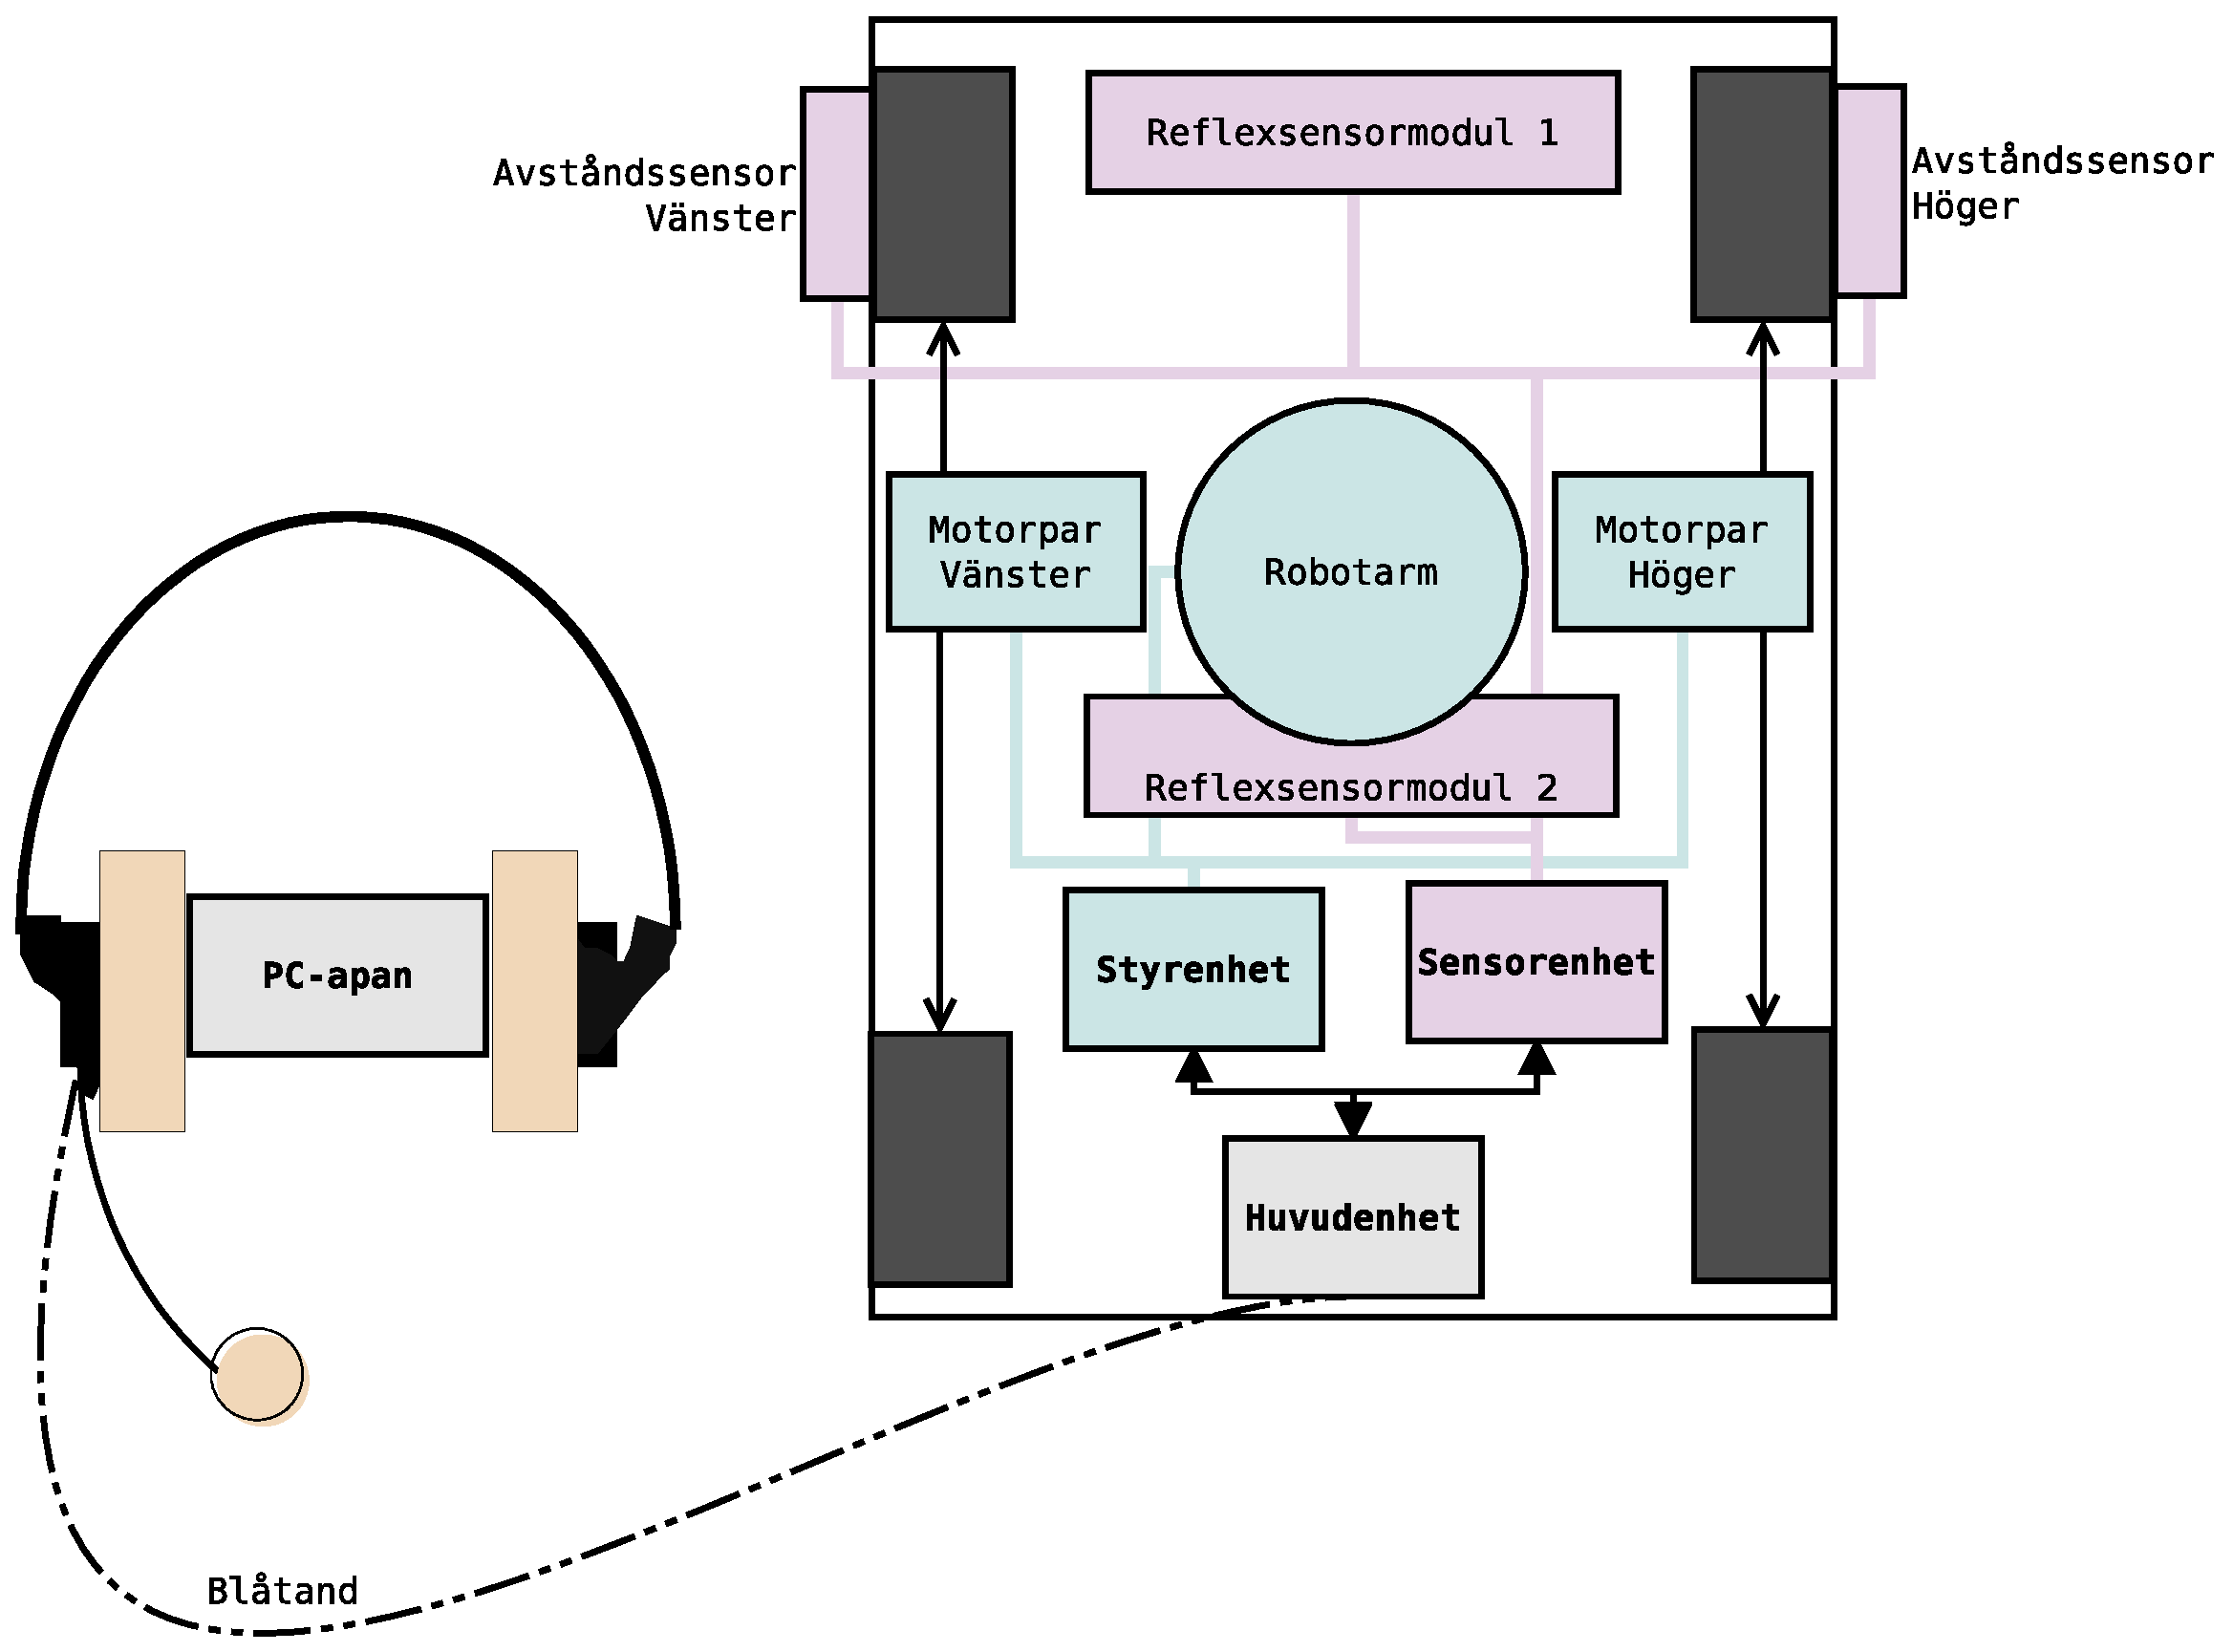
\includegraphics[scale=0.4]{grafik/system-oversikt}
	\caption{Översikt av systemet} \label{system-oversikt}
\end{figure}

PCenheten innefattar ett grafiskt gränssnitt där man kan se debugmeddelanden, sensordata, motorhastigheter och armens position. I det grafiska gränssnittet finns reglage för att bestämma om systemet är i sitt manuella eller autonoma läge. När systemet är i sitt manuella läge styrs det med två joysticks via det grafiska gränssnittet.

Huvudenheten innehåller robotens intelligens, den tar beslut om vad som ska göras beroende på om roboten är i sitt manuella eller autonoma läge. I det autonoma läget är det i huvudenheten all styrlogik finns som säger vart roboten är och vad den ska göra. Det är även där regleringen ligger som ser till att roboten följer banan.

Sensorenheten förser huvudenheten med sensordata.

Styrenheten tar instruktioner från huvudenheten och ser till att motorer och servon utför dessa.

\section{Kommunikation}

\todo{Överväger att lägga figur \ref{kommunikation-oversikt} i Systemet och protokollen under varje enhet.}

\begin{figure}[h!]
	\centering
	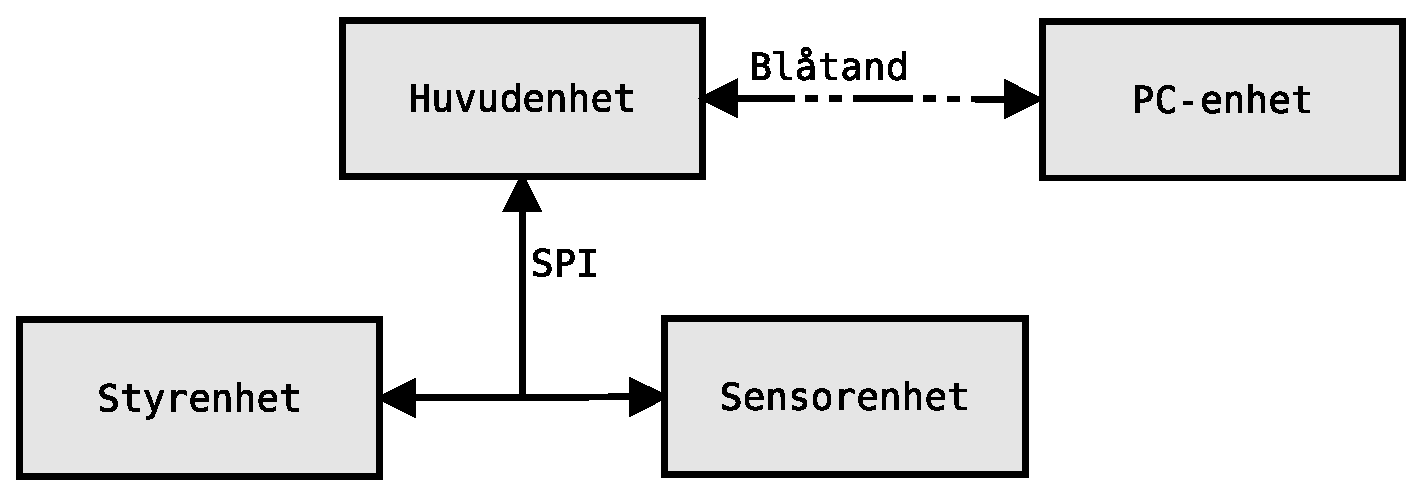
\includegraphics[scale=0.4]{grafik/kommunikation-oversikt}
	\caption{Översikt systemets kommunikationskanaler} \label{kommunikation-oversikt}
\end{figure}

Figur \ref{kommunikation-oversikt} ger en översikt av vilka moduler som kommunicerar med varandra och på vilket sätt detta sker. Styrenheten och Sensorenheten använder samma SPI-buss fast med olika Slave Select-pinnar.

\subsection{PC-enhet $\longleftrightarrow$ Huvudenhet}

PC-enheten och Huvudenheten kommunicerar över Blåtand.
\todo{Hur set det här protokollet ut i verkligheten?}

\subsection{Huvudenhet $\longleftrightarrow$ Styrenhet}

Huvudenheten kommunicerar med Styrenheten över SPI. Storleken på en instruktion är antingen fyra eller sju bytes lång. För att förebygga synkroniseringsproblem skickas först två startbytes bestående av hexadecimalt $0xff$ följt av längden på instruktionen (startbytesen och längdbyten räknas ej med). Därefter följer instruktionsbyten som består av två delar. De fyra högsta bitarna anger vilken instruktion som ska utföras enligt tabell \ref{protokoll:pc-motor-tabell}, och de fyra lägsta vilket servo eller motorpar instruktionen rör enligt tabell \ref{protokoll:pc-motor-adress-tabell}. I fallet att instruktionen är \textit{Sätt register A till D} krävs dessutom två databytes.

Då ett motorpar adresseras anger den minsta biten i den första databyten vilken riktning motorparet skall röra sig. $0$ anger framåt, $1$ bakåt \todo{Stämmer?}. Den andra databyten anger vilken fart vi vill att motorerna skall röra sig i. Notera att motorerna sätts med kommandot $Sätt register A till D$.

De servon vi arbetar med har en upplösning på 10 bitar både för position och hastighet. Vi måste alltså ha två databytes när vi vill ändra någon egenskap hos dessa. De två minsta bitarna i den första databyten är de två högsta bitarna och därefter följer den andra databyten.

\todo{Tabell för att illustrera bitar hit och dit?}

\subsection{Instruktionslista}

\begin{table}[h!]
	\centering
	\begin{tabularx}{\textwidth}{| l | l | X |}
		\hline
		\textbf{Instruktion} & \textbf{Argument} & \textbf{Beskrivning} \\\hline
		{0000} & {} & {Stoppa samtliga servon och motorer \todo{Behöver implementeras}} \\\hline
		{0001} & {A, D} & {Sätt register A till D} \\\hline
		{0010} & {A} & {Utför givna kommandon för A} \\\hline
		{0011} & {A, D} & {Sätt servohastighet för A till D} \\\hline
		{0100} & {A} & {Returnera Status för A \todo{Implementera?}} \\\hline
	\end{tabularx}
	\caption{Kommandon från huvudenhet till styrenhet \todo{Stämmer tabellen?}} \label{protokoll:pc-motor-tabell}
\end{table}

\begin{table}[h!]
	\centering
	\begin{tabularx}{\textwidth}{| l | X |}
		\hline
		\textbf{Adress} & \textbf{Beskrivning} \\\hline
		{0000} & {Höger hjulpar} \\\hline
		{0001} & {Vänster hjulpar} \\\hline
		{0010} & {Arm axel 1} \\\hline
		{0100} & {Arm axel 2} \\\hline
		{0110} & {Arm axel 3} \\\hline
		{1000} & {Arm axel 4} \\\hline
		{1011} & {Arm axel 5 (\textit{gripklo})} \\\hline
		{1100} & {Samtliga motorer} \\\hline
		{1101} & {Samtliga servon} \\\hline
		{1111} & {Samtliga motorer och servon} \\\hline
	\end{tabularx}
	\caption{Adresser för adressering till styrenhet} \label{protokoll:pc-motor-adress-tabell}
\end{table}

\subsection{Huvudenhet $\longleftrightarrow$ Sensorenhet}

Huvudenheten kommunicerar med Sensorenheten över SPI. Protokollet mellan dessa moduler är väldigt primitivt då det endast finns en instruktion, returnera sensordata för begärd sensor. Instruktionen anges av de 4 högsta bitarna av instruktionsbyten enligt tabell \ref{protokoll:huvud-sensor}. Huvudenhetens begäran är då bara på en enda databyte och Sensorenheten svarar med de 8 högsta bitarna för den efterfrågade sensorn. Vilken sensor som enheten returnerar data för anges av de 4 minsta bitarna i instruktionsbyten enligt tabell \ref{protokoll:huvud-sensor-adress}.

\subsection{Instruktionslista}

\begin{table}[h!]
	\centering
	\begin{tabularx}{\textwidth}{| l | l | X |}
		\hline
		\textbf{Instruktion} & \textbf{Argument} & \textbf{Beskrivning} \\\hline
		{0000} & {A} & {Returnera sensordata för A} \\\hline
	\end{tabularx}
	\caption{Instruktion från huvudenhet till sensorenhet} \label{protokoll:huvud-sensor}
\end{table}

\begin{table}[h!]
	\centering
	\begin{tabularx}{\textwidth}{| l | X |}
		\hline
		\textbf{Adress} & \textbf{Beskrivning} \\\hline
		{0000} & {Linjesensor 1} \\\hline
		{0001} & {Linjesensor 2} \\\hline
		{0010} & {Linjesensor 3} \\\hline
		{0011} & {Linjesensor 4} \\\hline
		{0100} & {Linjesensor 5} \\\hline
		{0101} & {Linjesensor 6} \\\hline
		{0110} & {Linjesensor 7} \\\hline
		{0111} & {Linjesensor 8} \\\hline
		{1000} & {Linjesensor 9} \\\hline
		{1001} & {Linjesensor 10} \\\hline
		{1010} & {Linjesensor 11} \\\hline
		{1011} & {Avståndssensor Höger} \\\hline
		{1100} & {Avståndssensor Vänster} \\\hline
	\end{tabularx}
	\caption{Adresser för instruktioner till sensorenhet} \label{protokoll:huvud-sensor-adress}
\end{table}

\section{Teori}
I projektet ingår främst två större teoretiska beräkningsmoment. Vi måste reglera utdatan till motorerna för att roboten skall följa linjen. Vidare vill vi kunna använda enklare koordinater för att tala om vart i rummet armen befinner sig, och vi behöver således kunna konvertera $(x,y,z)$-koordinater till vinklar för armens axlar.

\subsection{Reglering}
För att följa banan måste vi reglera motorernas hastighet. Vi gör detta genom att beräkna ett fel och ändra motorernas hastighet proportionellt mot detta. Felet beräknas genom att vi i varje iteration beräknar vart tejpen befinner sig längs den främre linjesensorn. För att göra detta multiplicerar vi linjesensorvärdena med vikter, dividerar med summan av linjesensorvärdena och subtraherar sedan medianvärdet, vilket i det här fallet är $6$. Vi får ekvation \ref{eq1}.

\begin{equation} \label{eq1}
	Q_{fel}=6-\frac{\sum_{i=1}^{11}S_{n}*n}{\sum_{i=1}^{11}S_n}
\end{equation}

För att beräkna utsignalen använder vi felet $Q_{fel}$ och förändringen jämfört med förra iterationen ${\Delta}Q_{fel}$ tillsammans med konstanterna $P$ och $D$. Vi vet att regleringen körs med en uppdateringsfrekvens på 50Hz.

\begin{equation} \label{eq2}
	Q_{out}=(P*Q_{fel}+D*{\Delta}Q_{fel})*freq
\end{equation}

$Q_{out}$ i ekvationen ovan är den utsignal som används för att beräkna motorernas nya hastigheter.

\subsection{Styrning av arm}
Omvandlingen från $(x,y,z)$-koordinater till vinklar för armens servon sker på huvudenheten. På huvudenheten finns en pythonmodul \texttt{arm.py} som implementerar beräkningarna som beskrivs nedan. Den används i tre steg.
\begin{enumerate}
	\item Skapa en instans av \texttt{robotArm} som är en klass i \texttt{arm.py}.
	\item Använd funktionen \texttt{setAll} som tar in en lista som argument med följande innehåll \newline \texttt{[x,y,z,gripperAngle,gripperRotationsOffset,gripper]}.
	\item Använd funktionen \texttt{getServoValues} som returnerar en lista med alla servons vinklar i form av 10-bitars heltal.
\end{enumerate}

GripperAngle är gripklons vinkel mot marken, gripperRotationsOffset är en offset på gripklons vinkel i förhållande till leden som gripklon är fäst i och gripper är hur mycket gripklon klämmer.

I listan som returneras är första värdet till armens bas, det andra är till $A1$, det tredje är till $A2$, det fjärde till $A3$, det femte till klons rotation och det sjätte till klons grepp.

\begin{figure}[h!]
	\centerline{% Graphic for TeX using PGF
% Title: /home/martin/Diagram1.dia
% Creator: Dia v0.97.2
% CreationDate: Sun Oct 12 18:13:42 2014
% For: martin
% \usepackage{tikz}
% The following commands are not supported in PSTricks at present
% We define them conditionally, so when they are implemented,
% this pgf file will use them.
\ifx\du\undefined
  \newlength{\du}
\fi
\setlength{\du}{15\unitlength}
\begin{tikzpicture}
\pgftransformxscale{1.000000}
\pgftransformyscale{-1.000000}
\definecolor{dialinecolor}{rgb}{0.000000, 0.000000, 0.000000}
\pgfsetstrokecolor{dialinecolor}
\definecolor{dialinecolor}{rgb}{1.000000, 1.000000, 1.000000}
\pgfsetfillcolor{dialinecolor}
\pgfsetlinewidth{0.100000\du}
\pgfsetdash{}{0pt}
\pgfsetdash{}{0pt}
\pgfsetmiterjoin
\definecolor{dialinecolor}{rgb}{1.000000, 1.000000, 1.000000}
\pgfsetfillcolor{dialinecolor}
\fill (3.300000\du,-2.250000\du)--(3.300000\du,4.212500\du)--(8.950000\du,4.212500\du)--(8.950000\du,-2.250000\du)--cycle;
\definecolor{dialinecolor}{rgb}{0.000000, 0.000000, 0.000000}
\pgfsetstrokecolor{dialinecolor}
\draw (3.300000\du,-2.250000\du)--(3.300000\du,4.212500\du)--(8.950000\du,4.212500\du)--(8.950000\du,-2.250000\du)--cycle;
\pgfsetlinewidth{0.100000\du}
\pgfsetdash{}{0pt}
\pgfsetdash{}{0pt}
\pgfsetbuttcap
\pgfsetmiterjoin
\pgfsetlinewidth{0.100000\du}
\pgfsetbuttcap
\pgfsetmiterjoin
\pgfsetdash{}{0pt}
\definecolor{dialinecolor}{rgb}{1.000000, 1.000000, 1.000000}
\pgfsetfillcolor{dialinecolor}
\pgfpathellipse{\pgfpoint{6.137500\du}{0.787500\du}}{\pgfpoint{1.537500\du}{0\du}}{\pgfpoint{0\du}{1.537500\du}}
\pgfusepath{fill}
\definecolor{dialinecolor}{rgb}{0.000000, 0.000000, 0.000000}
\pgfsetstrokecolor{dialinecolor}
\pgfpathellipse{\pgfpoint{6.137500\du}{0.787500\du}}{\pgfpoint{1.537500\du}{0\du}}{\pgfpoint{0\du}{1.537500\du}}
\pgfusepath{stroke}
\pgfsetbuttcap
\pgfsetmiterjoin
\pgfsetdash{}{0pt}
\definecolor{dialinecolor}{rgb}{0.000000, 0.000000, 0.000000}
\pgfsetstrokecolor{dialinecolor}
\pgfpathellipse{\pgfpoint{6.137500\du}{0.787500\du}}{\pgfpoint{1.537500\du}{0\du}}{\pgfpoint{0\du}{1.537500\du}}
\pgfusepath{stroke}
\pgfsetlinewidth{0.100000\du}
\pgfsetdash{}{0pt}
\pgfsetdash{}{0pt}
\pgfsetbuttcap
{
\definecolor{dialinecolor}{rgb}{0.000000, 0.000000, 0.000000}
\pgfsetfillcolor{dialinecolor}
% was here!!!
\definecolor{dialinecolor}{rgb}{0.000000, 0.000000, 0.000000}
\pgfsetstrokecolor{dialinecolor}
\draw (7.231647\du,-0.360394\du)--(9.700000\du,-2.950000\du);
}
\pgfsetlinewidth{0.100000\du}
\pgfsetdash{}{0pt}
\pgfsetdash{}{0pt}
\pgfsetbuttcap
{
\definecolor{dialinecolor}{rgb}{0.000000, 0.000000, 0.000000}
\pgfsetfillcolor{dialinecolor}
% was here!!!
\pgfsetarrowsend{to}
\definecolor{dialinecolor}{rgb}{0.000000, 0.000000, 0.000000}
\pgfsetstrokecolor{dialinecolor}
\draw (9.850000\du,-3.000000\du)--(14.300000\du,-2.950000\du);
}
\pgfsetlinewidth{0.100000\du}
\pgfsetdash{}{0pt}
\pgfsetdash{}{0pt}
\pgfsetbuttcap
{
\definecolor{dialinecolor}{rgb}{0.000000, 0.000000, 0.000000}
\pgfsetfillcolor{dialinecolor}
% was here!!!
\pgfsetarrowsend{to}
\definecolor{dialinecolor}{rgb}{0.000000, 0.000000, 0.000000}
\pgfsetstrokecolor{dialinecolor}
\draw (9.750000\du,-3.187500\du)--(9.700000\du,-7.637500\du);
}
% setfont left to latex
\definecolor{dialinecolor}{rgb}{0.000000, 0.000000, 0.000000}
\pgfsetstrokecolor{dialinecolor}
\node[anchor=west] at (14.650000\du,-2.787500\du){X-led};
% setfont left to latex
\definecolor{dialinecolor}{rgb}{0.000000, 0.000000, 0.000000}
\pgfsetstrokecolor{dialinecolor}
\node[anchor=west] at (9.700000\du,-7.737500\du){Y-led};
\end{tikzpicture}
}
	\caption{Armens koordinatsystem i förhållande till roboten. Upp är robotens färdriktning}
\end{figure}

\begin{figure}[h!]
	\centerline{% Graphic for TeX using PGF
% Title: /home/martin/Diagram1.dia
% Creator: Dia v0.97.2
% CreationDate: Sun Oct 12 20:23:47 2014
% For: martin
% \usepackage{tikz}
% The following commands are not supported in PSTricks at present
% We define them conditionally, so when they are implemented,
% this pgf file will use them.
\ifx\du\undefined
  \newlength{\du}
\fi
\setlength{\du}{15\unitlength}
\begin{tikzpicture}
\pgftransformxscale{1.000000}
\pgftransformyscale{-1.000000}
\definecolor{dialinecolor}{rgb}{0.000000, 0.000000, 0.000000}
\pgfsetstrokecolor{dialinecolor}
\definecolor{dialinecolor}{rgb}{1.000000, 1.000000, 1.000000}
\pgfsetfillcolor{dialinecolor}
\pgfsetlinewidth{0.100000\du}
\pgfsetdash{}{0pt}
\pgfsetdash{}{0pt}
\pgfsetbuttcap
{
\definecolor{dialinecolor}{rgb}{0.000000, 0.000000, 0.000000}
\pgfsetfillcolor{dialinecolor}
% was here!!!
\definecolor{dialinecolor}{rgb}{0.000000, 0.000000, 0.000000}
\pgfsetstrokecolor{dialinecolor}
\draw (3.650000\du,5.762500\du)--(7.900000\du,-1.587500\du);
}
\pgfsetlinewidth{0.100000\du}
\pgfsetdash{}{0pt}
\pgfsetdash{}{0pt}
\pgfsetbuttcap
{
\definecolor{dialinecolor}{rgb}{0.000000, 0.000000, 0.000000}
\pgfsetfillcolor{dialinecolor}
% was here!!!
\definecolor{dialinecolor}{rgb}{0.000000, 0.000000, 0.000000}
\pgfsetstrokecolor{dialinecolor}
\draw (7.850000\du,-1.537500\du)--(17.900000\du,-1.487500\du);
}
\pgfsetlinewidth{0.100000\du}
\pgfsetdash{}{0pt}
\pgfsetdash{}{0pt}
\pgfsetbuttcap
{
\definecolor{dialinecolor}{rgb}{0.000000, 0.000000, 0.000000}
\pgfsetfillcolor{dialinecolor}
% was here!!!
\definecolor{dialinecolor}{rgb}{0.000000, 0.000000, 0.000000}
\pgfsetstrokecolor{dialinecolor}
\draw (17.850000\du,-1.437500\du)--(20.900000\du,2.962500\du);
}
\pgfsetlinewidth{0.100000\du}
\pgfsetdash{{1.000000\du}{1.000000\du}}{0\du}
\pgfsetdash{{1.000000\du}{1.000000\du}}{0\du}
\pgfsetbuttcap
{
\definecolor{dialinecolor}{rgb}{0.000000, 0.000000, 0.000000}
\pgfsetfillcolor{dialinecolor}
% was here!!!
\definecolor{dialinecolor}{rgb}{0.000000, 0.000000, 0.000000}
\pgfsetstrokecolor{dialinecolor}
\draw (3.600000\du,6.162500\du)--(3.600000\du,-7.087500\du);
}
\pgfsetlinewidth{0.100000\du}
\pgfsetdash{{1.000000\du}{1.000000\du}}{0\du}
\pgfsetdash{{1.000000\du}{1.000000\du}}{0\du}
\pgfsetbuttcap
{
\definecolor{dialinecolor}{rgb}{0.000000, 0.000000, 0.000000}
\pgfsetfillcolor{dialinecolor}
% was here!!!
\definecolor{dialinecolor}{rgb}{0.000000, 0.000000, 0.000000}
\pgfsetstrokecolor{dialinecolor}
\draw (3.700000\du,6.212500\du)--(27.500000\du,6.062500\du);
}
\pgfsetlinewidth{0.100000\du}
\pgfsetdash{}{0pt}
\pgfsetdash{}{0pt}
\pgfsetbuttcap
{
\definecolor{dialinecolor}{rgb}{0.000000, 0.000000, 0.000000}
\pgfsetfillcolor{dialinecolor}
% was here!!!
\definecolor{dialinecolor}{rgb}{0.000000, 0.000000, 0.000000}
\pgfsetstrokecolor{dialinecolor}
\pgfpathmoveto{\pgfpoint{6.049937\du}{6.212702\du}}
\pgfpatharc{18}{-65}{2.110604\du and 2.110604\du}
\pgfusepath{stroke}
}
\pgfsetlinewidth{0.100000\du}
\pgfsetdash{}{0pt}
\pgfsetdash{}{0pt}
\pgfsetbuttcap
{
\definecolor{dialinecolor}{rgb}{0.000000, 0.000000, 0.000000}
\pgfsetfillcolor{dialinecolor}
% was here!!!
\definecolor{dialinecolor}{rgb}{0.000000, 0.000000, 0.000000}
\pgfsetstrokecolor{dialinecolor}
\pgfpathmoveto{\pgfpoint{6.949854\du}{0.062444\du}}
\pgfpatharc{112}{9}{2.148827\du and 2.148827\du}
\pgfusepath{stroke}
}
\pgfsetlinewidth{0.100000\du}
\pgfsetdash{}{0pt}
\pgfsetdash{}{0pt}
\pgfsetbuttcap
{
\definecolor{dialinecolor}{rgb}{0.000000, 0.000000, 0.000000}
\pgfsetfillcolor{dialinecolor}
% was here!!!
\definecolor{dialinecolor}{rgb}{0.000000, 0.000000, 0.000000}
\pgfsetstrokecolor{dialinecolor}
\pgfpathmoveto{\pgfpoint{16.550022\du}{-1.537549\du}}
\pgfpatharc{205}{42}{1.170625\du and 1.170625\du}
\pgfusepath{stroke}
}
\pgfsetlinewidth{0.100000\du}
\pgfsetdash{{1.000000\du}{1.000000\du}}{0\du}
\pgfsetdash{{1.000000\du}{1.000000\du}}{0\du}
\pgfsetbuttcap
{
\definecolor{dialinecolor}{rgb}{0.000000, 0.000000, 0.000000}
\pgfsetfillcolor{dialinecolor}
% was here!!!
\definecolor{dialinecolor}{rgb}{0.000000, 0.000000, 0.000000}
\pgfsetstrokecolor{dialinecolor}
\draw (18.200000\du,2.962500\du)--(27.950000\du,2.912500\du);
}
\pgfsetlinewidth{0.100000\du}
\pgfsetdash{}{0pt}
\pgfsetdash{}{0pt}
\pgfsetbuttcap
{
\definecolor{dialinecolor}{rgb}{0.000000, 0.000000, 0.000000}
\pgfsetfillcolor{dialinecolor}
% was here!!!
\definecolor{dialinecolor}{rgb}{0.000000, 0.000000, 0.000000}
\pgfsetstrokecolor{dialinecolor}
\pgfpathmoveto{\pgfpoint{19.950016\du}{1.812506\du}}
\pgfpatharc{292}{159}{0.849480\du and 0.849480\du}
\pgfusepath{stroke}
}
% setfont left to latex
\definecolor{dialinecolor}{rgb}{0.000000, 0.000000, 0.000000}
\pgfsetstrokecolor{dialinecolor}
\node[anchor=west] at (0.500000\du,6.112500\du){P0=(0,0)};
% setfont left to latex
\definecolor{dialinecolor}{rgb}{0.000000, 0.000000, 0.000000}
\pgfsetstrokecolor{dialinecolor}
\node[anchor=west] at (5.650000\du,4.062500\du){A1};
% setfont left to latex
\definecolor{dialinecolor}{rgb}{0.000000, 0.000000, 0.000000}
\pgfsetstrokecolor{dialinecolor}
\node[anchor=west] at (8.900000\du,0.862500\du){A2};
% setfont left to latex
\definecolor{dialinecolor}{rgb}{0.000000, 0.000000, 0.000000}
\pgfsetstrokecolor{dialinecolor}
\node[anchor=west] at (16.350000\du,0.762500\du){A3};
% setfont left to latex
\definecolor{dialinecolor}{rgb}{0.000000, 0.000000, 0.000000}
\pgfsetstrokecolor{dialinecolor}
\node[anchor=west] at (14.800000\du,2.562500\du){};
% setfont left to latex
\definecolor{dialinecolor}{rgb}{0.000000, 0.000000, 0.000000}
\pgfsetstrokecolor{dialinecolor}
\node[anchor=west] at (18.150000\du,1.812500\du){};
% setfont left to latex
\definecolor{dialinecolor}{rgb}{0.000000, 0.000000, 0.000000}
\pgfsetstrokecolor{dialinecolor}
\node[anchor=west] at (17.850000\du,2.062500\du){A4};
% setfont left to latex
\definecolor{dialinecolor}{rgb}{0.000000, 0.000000, 0.000000}
\pgfsetstrokecolor{dialinecolor}
\node[anchor=west] at (4.850000\du,1.162500\du){L1};
% setfont left to latex
\definecolor{dialinecolor}{rgb}{0.000000, 0.000000, 0.000000}
\pgfsetstrokecolor{dialinecolor}
\node[anchor=west] at (12.600000\du,-2.287500\du){L2};
% setfont left to latex
\definecolor{dialinecolor}{rgb}{0.000000, 0.000000, 0.000000}
\pgfsetstrokecolor{dialinecolor}
\node[anchor=west] at (20.050000\du,0.362500\du){L3};
% setfont left to latex
\definecolor{dialinecolor}{rgb}{0.000000, 0.000000, 0.000000}
\pgfsetstrokecolor{dialinecolor}
\node[anchor=west] at (7.100000\du,-2.337500\du){P1=(W1,Z1)};
% setfont left to latex
\definecolor{dialinecolor}{rgb}{0.000000, 0.000000, 0.000000}
\pgfsetstrokecolor{dialinecolor}
\node[anchor=west] at (18.175000\du,-2.337500\du){P2=(W2,Z2)};
% setfont left to latex
\definecolor{dialinecolor}{rgb}{0.000000, 0.000000, 0.000000}
\pgfsetstrokecolor{dialinecolor}
\node[anchor=west] at (20.825000\du,3.912500\du){P3=(W,Z)};
% setfont left to latex
\definecolor{dialinecolor}{rgb}{0.000000, 0.000000, 0.000000}
\pgfsetstrokecolor{dialinecolor}
\node[anchor=west] at (20.925000\du,-2.637500\du){};
\pgfsetlinewidth{0.100000\du}
\pgfsetdash{}{0pt}
\pgfsetdash{}{0pt}
\pgfsetbuttcap
{
\definecolor{dialinecolor}{rgb}{0.000000, 0.000000, 0.000000}
\pgfsetfillcolor{dialinecolor}
% was here!!!
\definecolor{dialinecolor}{rgb}{0.000000, 0.000000, 0.000000}
\pgfsetstrokecolor{dialinecolor}
\draw (3.675000\du,6.212500\du)--(17.725000\du,-1.487500\du);
}
% setfont left to latex
\definecolor{dialinecolor}{rgb}{0.000000, 0.000000, 0.000000}
\pgfsetstrokecolor{dialinecolor}
\node[anchor=west] at (11.775000\du,2.762500\du){HL};
% setfont left to latex
\definecolor{dialinecolor}{rgb}{0.000000, 0.000000, 0.000000}
\pgfsetstrokecolor{dialinecolor}
\node[anchor=west] at (3.225000\du,-8.087500\du){z};
% setfont left to latex
\definecolor{dialinecolor}{rgb}{0.000000, 0.000000, 0.000000}
\pgfsetstrokecolor{dialinecolor}
\node[anchor=west] at (27.125000\du,6.062500\du){w};
\pgfsetlinewidth{0.100000\du}
\pgfsetdash{}{0pt}
\pgfsetdash{}{0pt}
\pgfsetbuttcap
{
\definecolor{dialinecolor}{rgb}{0.000000, 0.000000, 0.000000}
\pgfsetfillcolor{dialinecolor}
% was here!!!
\definecolor{dialinecolor}{rgb}{0.000000, 0.000000, 0.000000}
\pgfsetstrokecolor{dialinecolor}
\pgfpathmoveto{\pgfpoint{8.425000\du}{6.212503\du}}
\pgfpatharc{358}{321}{3.739603\du and 3.739603\du}
\pgfusepath{stroke}
}
% setfont left to latex
\definecolor{dialinecolor}{rgb}{0.000000, 0.000000, 0.000000}
\pgfsetstrokecolor{dialinecolor}
\node[anchor=west] at (8.825000\du,4.762500\du){HA};
\end{tikzpicture}
}
	\caption{Armens vinklar}
\end{figure}

Omvandlingen sker på följande sätt där gripperRotationOffset och gripper ignoreras. Antag att roboten startar i $(X,Y,Z,GR)=(0,0,0,\pi/2)$.
Där $GR$(GripRadian) är vilken vinkel gripklon har till $z$-axeln.\newline
Vi omvandlar våra rum-koordinater till en vinkel och plankoordinater $X,Y,Z,GR\rightarrow A,W,Z,GR$. Där $A$ är armens vinkel mot positiva $x$-axeln och $W$ är armens utsträckning.
$$A=tan^{-1}(\dfrac{Y}{X}) $$
$$W=\sqrt{X^2+Y^2}$$
Genom denna omvandlingen så kan vi göra om detta till ett 2-dimensionellt problem istället för ett 3-dimensionellt problem. Vi får in $X$,$Y$,$Z$,$GR$ och ställer in robotens vinkel mot $x$-axelns positiva del och sedan ser vi till att roboten bara har rätt utsträckning och höjd.
$$P_4=(W,Z)$$
$$P_0=(0,0)$$
$$W_2=W-cos(GR)*L_3$$
$$Z_2=Z-sin(GR)*L_3$$
$$H_L=\sqrt{W_2^2+Z_2^2}$$
$$H_A=tan^{-1}(\dfrac{Z_2}{W_2})$$
Cosinussatsen ger:
$$A_1=cos^{-1}(\dfrac{L_1^2+H_L^2-L_2^2}{2*L_1*H_L})+H_A$$
$$W_1=cos(A_1)*L_1$$
$$Z_1=sin(A_1)*L_1$$
$$A_2=tan^{-1}(\dfrac{Z_2-Z_1}{W_2-W_1})-A_1$$
$$A_3=GR-D_2-D_3$$

Då är alla vinklar beräknade men servornas nollpunkter är inte på samma ställen som nollställena i beräkningarna ovanför. Så följande offset ställs in i grader:

\begin{itemize}
	\item $A0=A0+60$
	\item $A1=240-A1$
	\item $A2=240-A2$
	\item $A3=150-A3$
	\item $A4=240-A0+GripperRotationOffset$ (klons rotation beror på basens rotation)
	\item $A5$ har ingen offset
\end{itemize}

Dessa vinklar är nu i grader. Dessa multipliceras nu med $\frac{1024}{360}$ för att omvandla grader till 10-bitars binära tal, avrundas nedåt till heltal och kan nu användas direkt av styrenheten.

% Hur är PC-enheten designad?

\section{PC-enhet}
PCenheten är ett verktyg för att göra det enklare för användaren att använda GLORIA.

\subsection{Hårdvara}

\subsection{Mjukvara}

% Hur huvudenheten är designad

\section{Huvudenhet}

\todo{Vad fyller Huvudenheten för funktion?}

\subsection{Hårdvara}
Den hårdvara som ingår i huvudenheten består av en Beagleboard-xm. På denna sitter en Blåtands-enhet av typ \todo{Typ/modell av BT?} monterad för kommunikation med PCenheten. Denna är ansluten till styrenheten och sensorenheten med en flatkabel som innehåller SPI-busen.
\todo{Bild på BB?}

\subsection{Mjukvara}
Mjukvaran är uppdelad i fyra trådar. En maintråd som har hand om all styrlogik, en pctråd som hanterar all kommunikation med PC:n, en sensortråd som kontinuerligt uppdaterar huvudenhetens sensorvärden och en regulatortråd som har hand om regleringen så roboten kan följa banan utan problem. Alla dessa kommunicerar med varandra genom en global datastruktur som innehållar alla olika variabler som behöver delas. Kommandon från PC:n delas mellan pctråden och maintråden genom en kö.

Figur \ref{huvud-tradar} illustrerar dataflödet mellan huvudenhetens olika trådar. Värt att notera är att det finns en tråd dedikerad till vardera extern enhet som kommunicerar med huvudenheten.

\begin{figure}[h!]
	\centering
	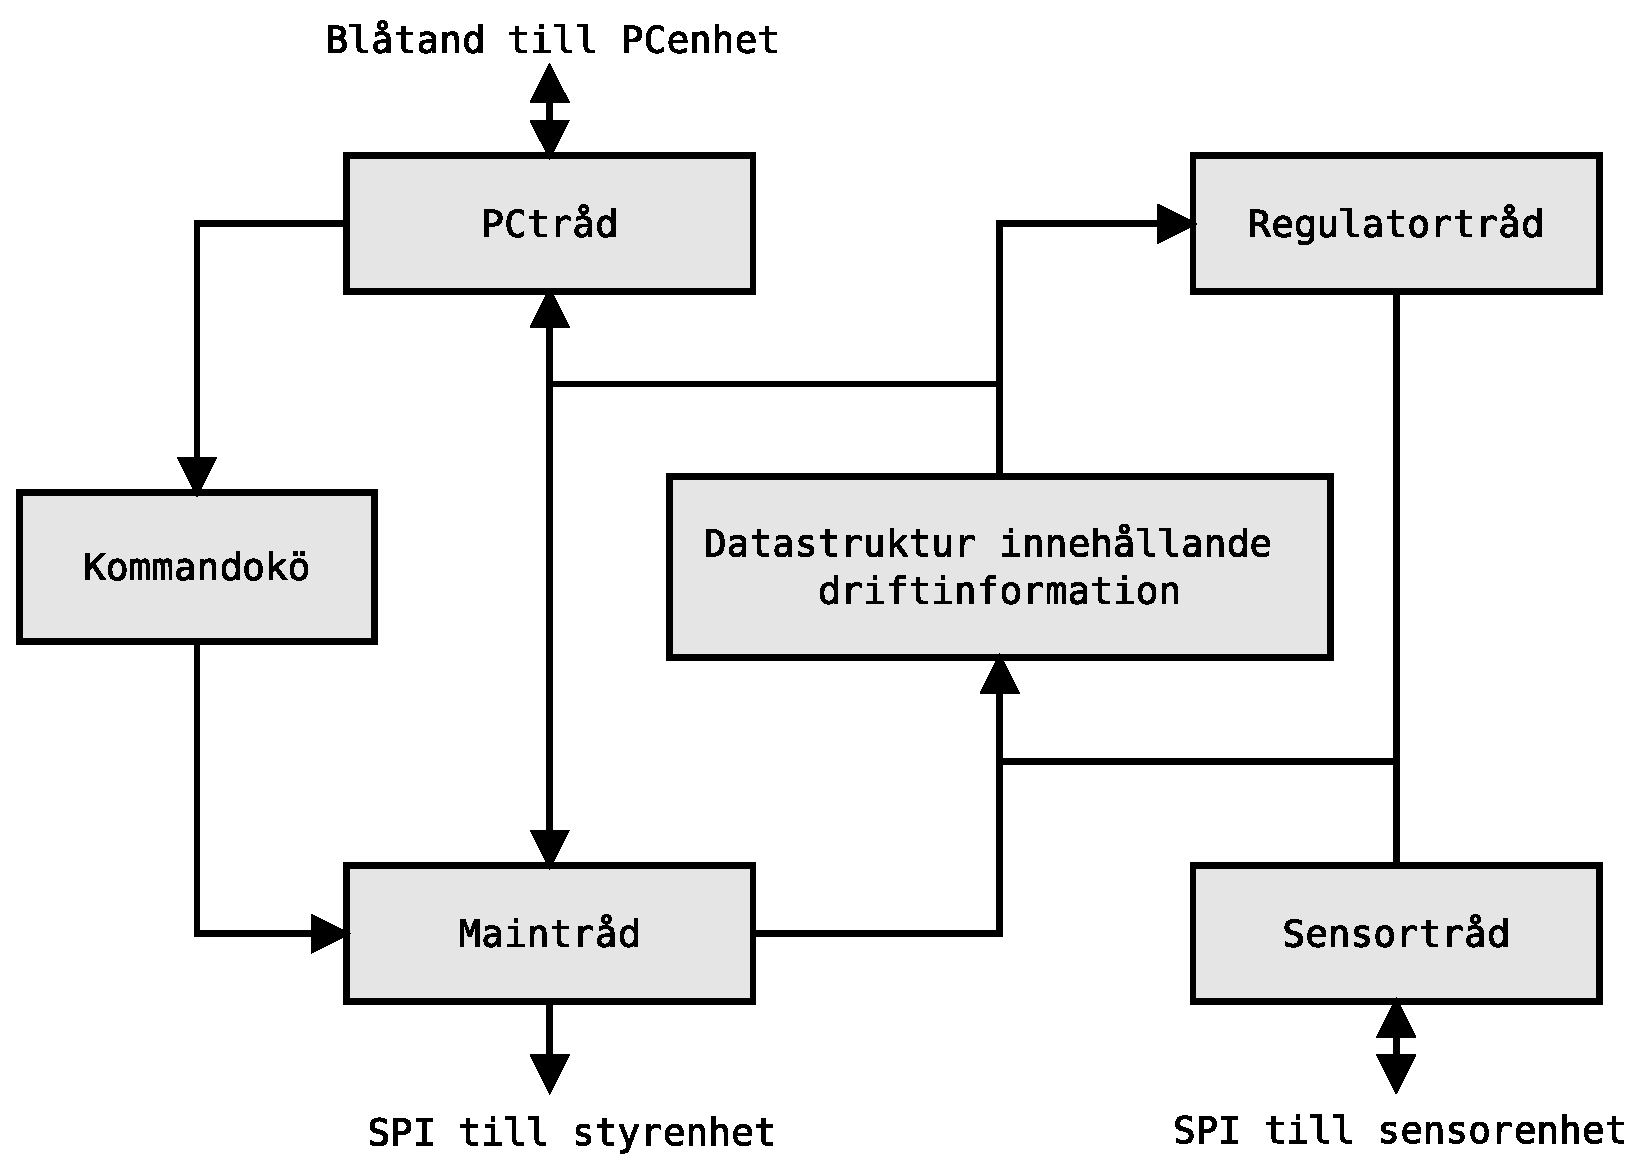
\includegraphics[scale=0.5]{grafik/huvud-tradar}
	\caption{Översikt över huvudenhetens trådar} \label{huvud-tradar}
\end{figure}

\subsubsection{Maintråd}
Maintråden är den tråd som ser till att vår robot faktiskt gör något med den information och de kommandon den tar emot från andra enheter. Tråden avgör vilket tillstånd systemet befinner sig i, om roboten skall köras autonomt beroende på sensordata eller om den bara ska utföra kommandon mottagna från PCenheten.

\paragraph{Tillstånd}

Systemet består av sex olika tillstånd, illustrerade i figur \ref{huvud-tillstand-diagram} och förklarade i tabell \ref{huvud-tillstand}. Det som inte syns i figuren är att systemet kan gå till tillståndet \texttt{MANUAL} även från de tre tillstånden \texttt{STATION FRONT}, \texttt{STATION CENTER} och \texttt{STATION BOTH} och i så fall kommer systemet även återgå till detta tidigare tillstånd från \texttt{MANUAL} då \texttt{autoMotor = True}. \todo{Formulering?}

\begin{figure}[h!]
	\centering
	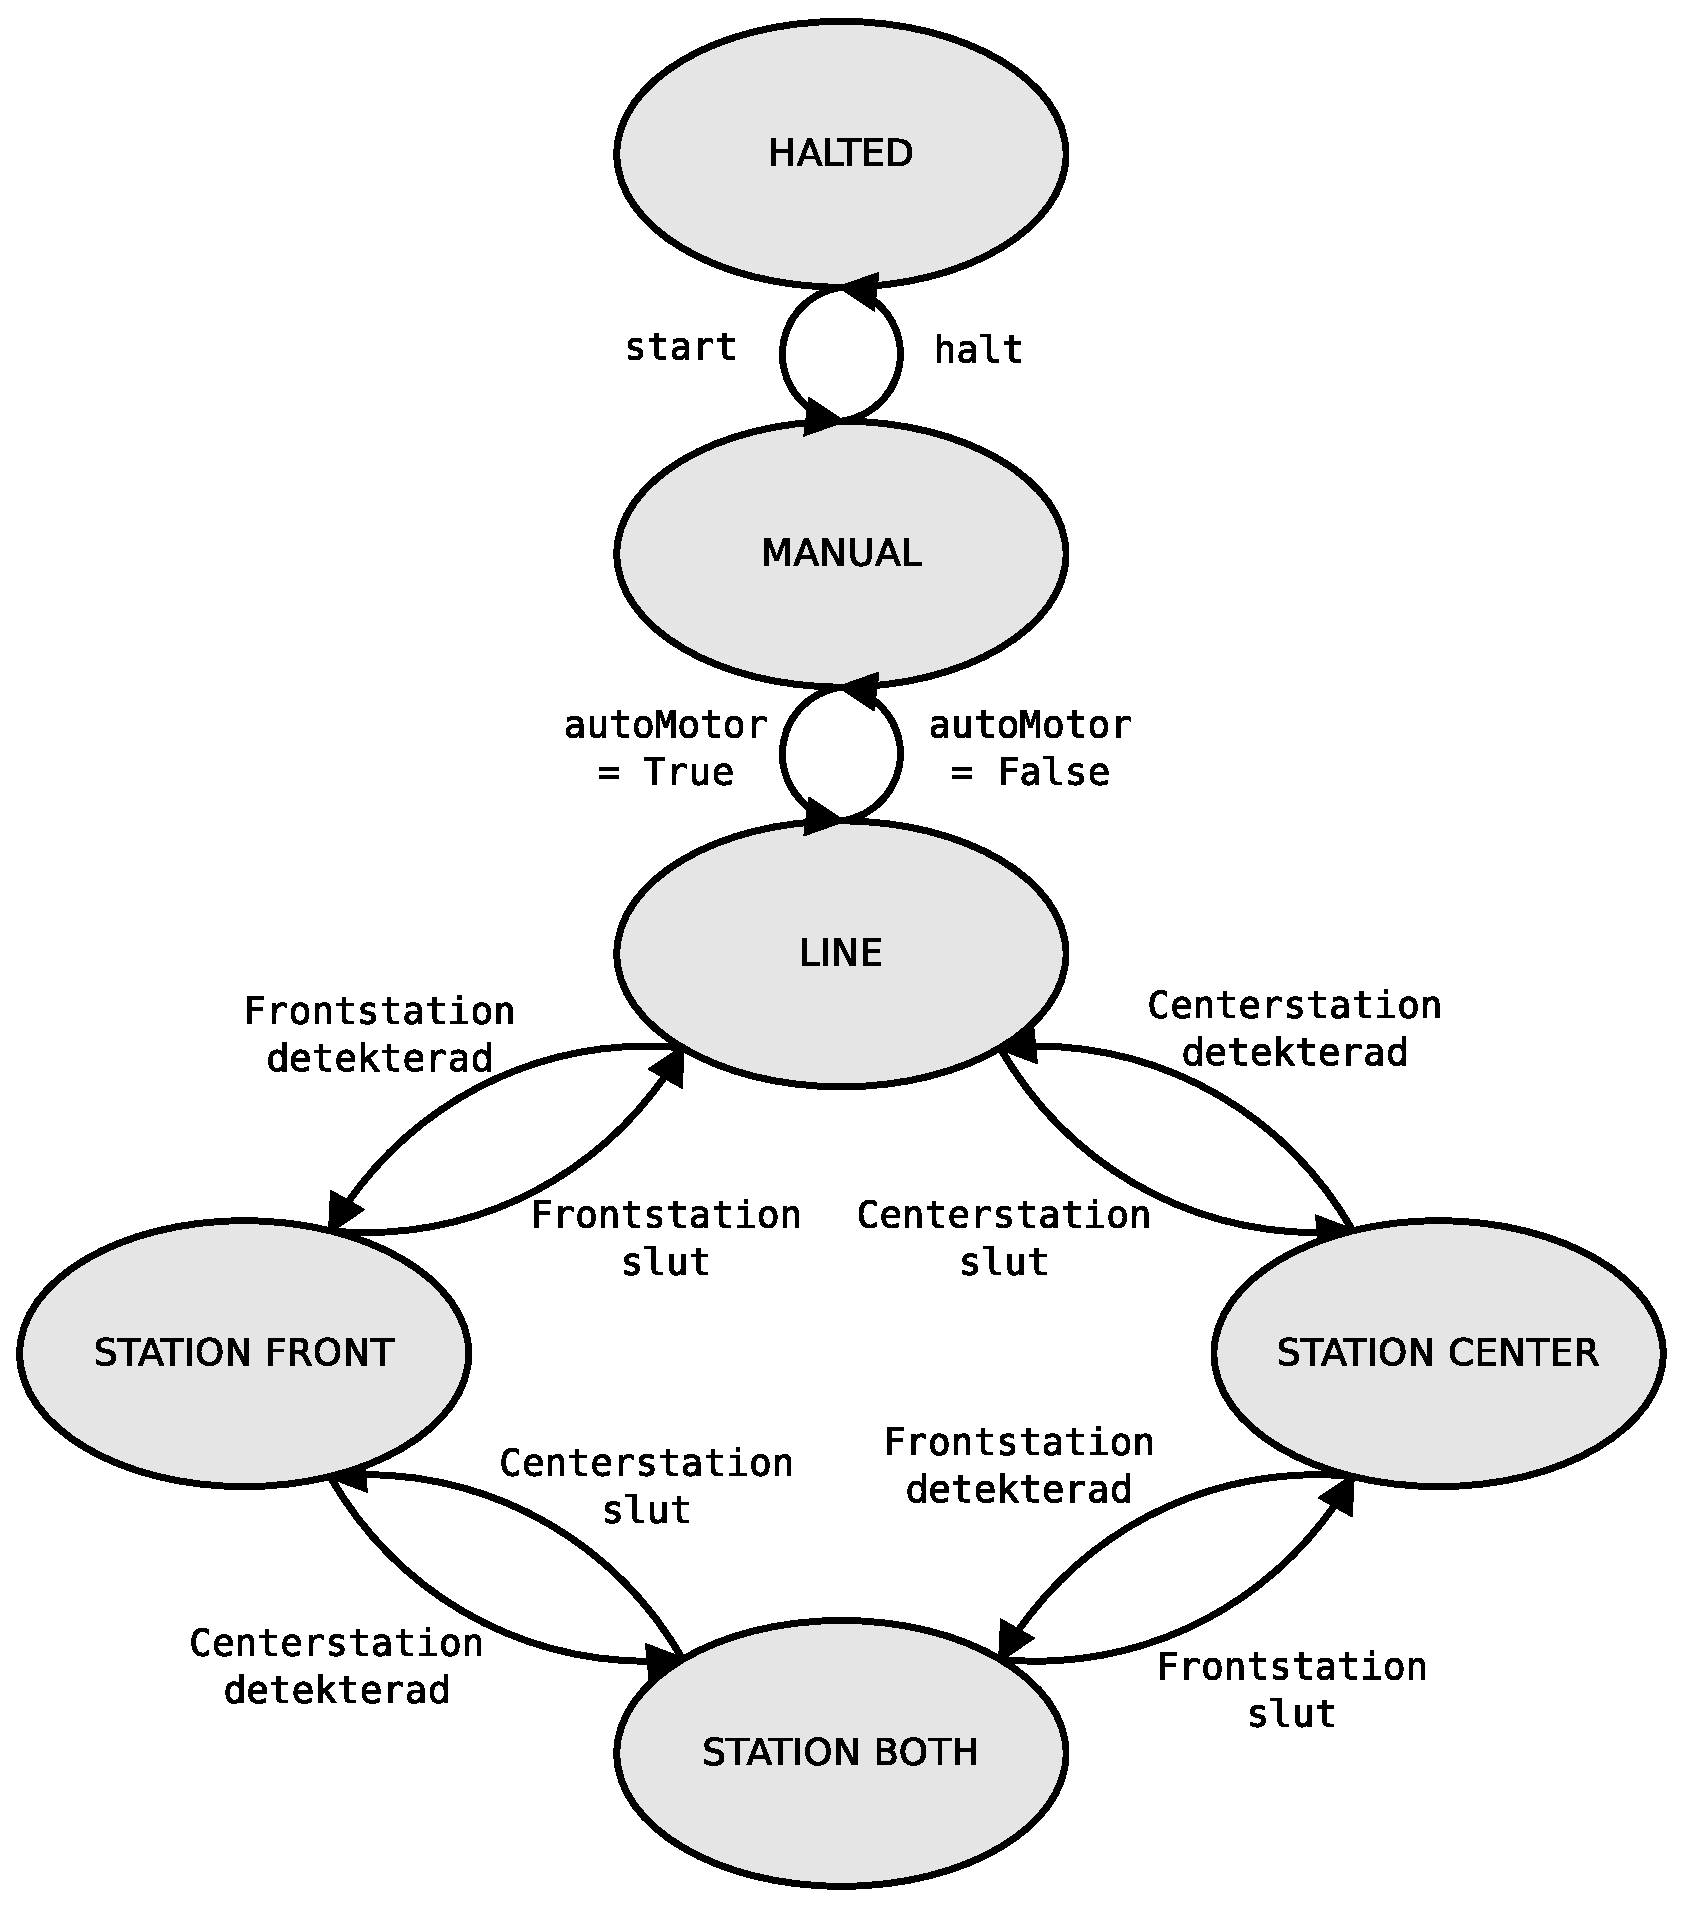
\includegraphics[scale=0.4]{grafik/huvud-tillstand}
	\caption{Översikt över maintrådens olika tillstånd} \label{huvud-tillstand-diagram}
\end{figure}

\begin{table}[h!]
	\centering
	\begin{tabularx}{\textwidth}{| l | X |}
		\hline
		{\textbf{Tillstånd}} & {\textbf{Beskrivning}} \\\hline
		{\texttt{HALTED}} & {Autonom och manuell styrning avstängd.} \\\hline
		{\texttt{MANUAL}} & {Systemet styrs manuellt.} \\\hline
		{\texttt{LINE}} & {Systemet kör autonomt.} \\\hline
		{\texttt{STATION FRONT}} & {Systemet har detekterat en station vid de främre sensorerna.} \\\hline
		{\texttt{STATION CENTER}} & {Systemet har detekterat en station vid de centrerade sensorerna.} \\\hline
		{\texttt{STATION BOTH}} & {Systemet har detekterat stationer vid både de främre och de centrerade sensorerna.} \\\hline
	\end{tabularx}
	\caption{Maintrådens olika tillstånd} \label{huvud-tillstand}
\end{table}

\paragraph{Detektion av stationer}

Det finns många potentiella felkällor vid detektion av stationer. Vi skulle kunna få en störning på utsignalen från våra analoga sensorer, underlaget kanske inte är helt homogent och regleringen skulle kunna få oss att momentant stå snett i en korsning. För att motverka dessa felkällor har vi olika typer av filter.

Vi filtrerar spikar från avståndssensorerna genom att vi lagrar de 10 senaste uppmätta värdena, viktar dessa med en binär skala ($D_{n}*2^{-n}$, där $D$ är uppmätta värden och $n$ är index i listan där $0$ är det senaste och $10$ det äldsta uppmätta värdet) och resultatet säger vi är det uppmätta avståndet.

Det finns inte samma möjlighet att att filtrera utdata från linjesensorerna på samma sätt, då vi även kan få fel på grund av reglering eller att en tejp i banan inte är helt rak. För varje iteration av sensordata från linjesensorn har vi en rad om 11 data. Istället för att filtrera vardera av dessa 11 data för sig, accepterar vi att ett fåtal av dessa data är avvikande. Den främre linjesensorn delas upp i segment enligt figur \ref{huvud-linjesensor} och för varje segment sätts ett krav för när detta segment kan betraktas detektera en faktisk tejp. För \textit{Höger} och \textit{Vänster} är kravet att tre av fyra sensorer är över tröskelvärdet. För \textit{Mitt} är kravet endast att en sensor är över tröskelvärdet. Endast två av sensorerna på den centrerade linjesensorn används, den har alltså endast två segment bestående av en sensor var, \textit{Center-höger} och \textit{Center-vänster}.

\begin{figure}[h!]
	\centering
	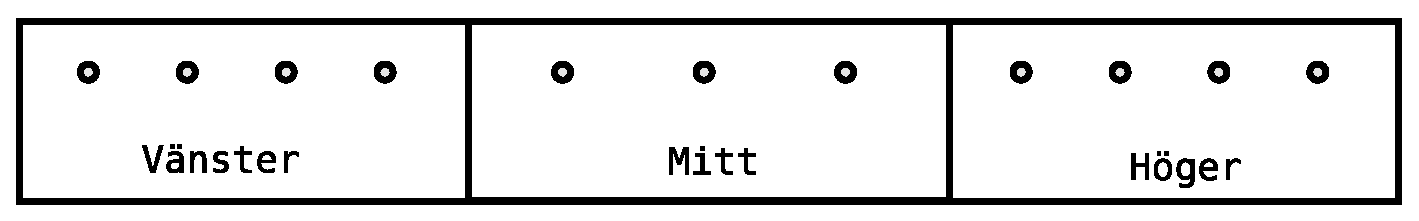
\includegraphics[scale=0.4]{grafik/huvud-linjesensor}
	\caption{Linjesensorn är uppdelad i segment} \label{huvud-linjesensor}
\end{figure}

För att inte upptäcka samma station flera gånger på grund av reglering eller sned bana och för att inte upptäcka en station i en korsning finns det även en mekanisk till. Varje iteration av sensordata sparas i en lista med de senaste sex iterationerna av sensorvärden. När vi sedan ska undersöka om det verkligen är en station vi är vid, går vi igenom alla sex iteration av sensordata. Om minst fyra av dessa rader av sensordata uppfyller kraven för en station, korsning eller ett avbrott i banan säger vi att så är fallet.

En station kännetecknas av att den ena av \textit{Höger} och \textit{Vänster} detekterar en tejp samtidigt som den inte gör det och vi också har tejp i \textit{Mitt}-segmentet. Skulle alla segment detektera en tejp har vi en korsande väg i banan som skall ignoreras och skulle inget segment detektera tejp har vi ett avbrott i banan.

Vi gör på motsvarande sätt för att detektera att en station är rakt under roboten. Där kräver vi att minst en sensor på \textit{Mitt}-segmentet på frontsensorn ska vara över tröskelvärdet i minst fyra av sex iterationer för att försäkra oss om att vi är på en någorlunda rak linje. Vidare kräver vi att de centrerade sensorerna ska vara över tröskelvärdet i minst fyra av de sex lagrade iterationerna.

\subsubsection{PCtråd}
PCtråden sätter upp en socket när den skapas och väntar på en inkommande anslutning från en PC. När den får en anslutning så väntar den på ett kommando.

\todo{Följande står redan i protokoll} Kommandot kommer som en textsträng på formatet \textit{;kommando=argument1,argument2;}. Om kommandot inte har några argument så ser strängen ut på följande sätt \textit{:"kommando"}.

Denna sträng görs om till en lista med följande utseende \textit{: ["kommando",["argument1","argument2"]]}.

Oftast tas flera kommandon emot samtidigt och PCtråden gör om dessa till en lista av kommandon som den går igenom och behandlar ett efter ett. Får man till exempel in två kommandon om sätta motorhastigheten så ser tillvägagångssättet ut på följande sätt:
\begin{enumerate}
\item ";motorSpeed=speed1,speed2;motorspeed=speed3;speed4;" tas emot
\item detta görs om till [["motorspeed",["speed1","speed2"]],["motorSpeed",["speed3","speed4"]]]
\item det första kommandot behandlas genom att argumenten omvandlas till heltal, motorernas hastighet uppdateras i dictionaryt och kommandot läggs till i kön så maintråden vet att den ska skicka ut kommandot.
\item nästa kommando behandlas på samma sätt men om speed1=speed3 och speed2=speed4 så ignoreras kommandot då det inte påverkar hastigheterna. \todo{Om speed1 != speed3, skrivs speed1 över? Skickar maintråden speed3 2 ggr?}
\end{enumerate}

\subsubsection{Sensortråd}
Sensortråden hämtar data från Sensorenheten med en given uppdateringsfrekvens. De hämtade sensorvärdena lagras i den globala datastrukturen.
\todo{Normaliserar filterar sensordata? Uppdateringsfrekvens, varför?}

\subsubsection{Regulatortråd}
Regulatortråden använder data från linjesensorerna för att beräkna hur roboten behöver röra sig för att följa linjen. Detta görs sedan om till motsvarande motorhastigheter och lagras i den globala datastrukturen.

Regleringen utförs i en egen tråd för att säkerhetsställa att beräkningarna sker med jämna tidsintervall.

\todo{Detektion av stationer/avbrott/stationer. Smart reglator!}
\todo{Förklara beroende till sensortråd}

% Detaljer hur styrenheten är designad

\section{Styrenhet}

Styrenheten har till uppgift att ta kommandon från huvudenheten och producera utsignaler som motorer och servon kan förstå.

\subsection{Hårdvara}
Styrenheten består av en Atmega1284p, en tri-state-krets\cite{tristate}, två motorpar och en robotarm Trossenrobotics Reactor\cite{robotarm}. Styrenheten är ansluten till huvudenheten via samma 20-pinnars flatkabel som sensorenheten. Figur \ref{styr-oversikt} illustrerar grovt hur de är ihopkopplade. Bilaga \ref{kopplingsschema} visar mer detaljerat hur det är kopplat.

\begin{figure}[h!]
	\centering
	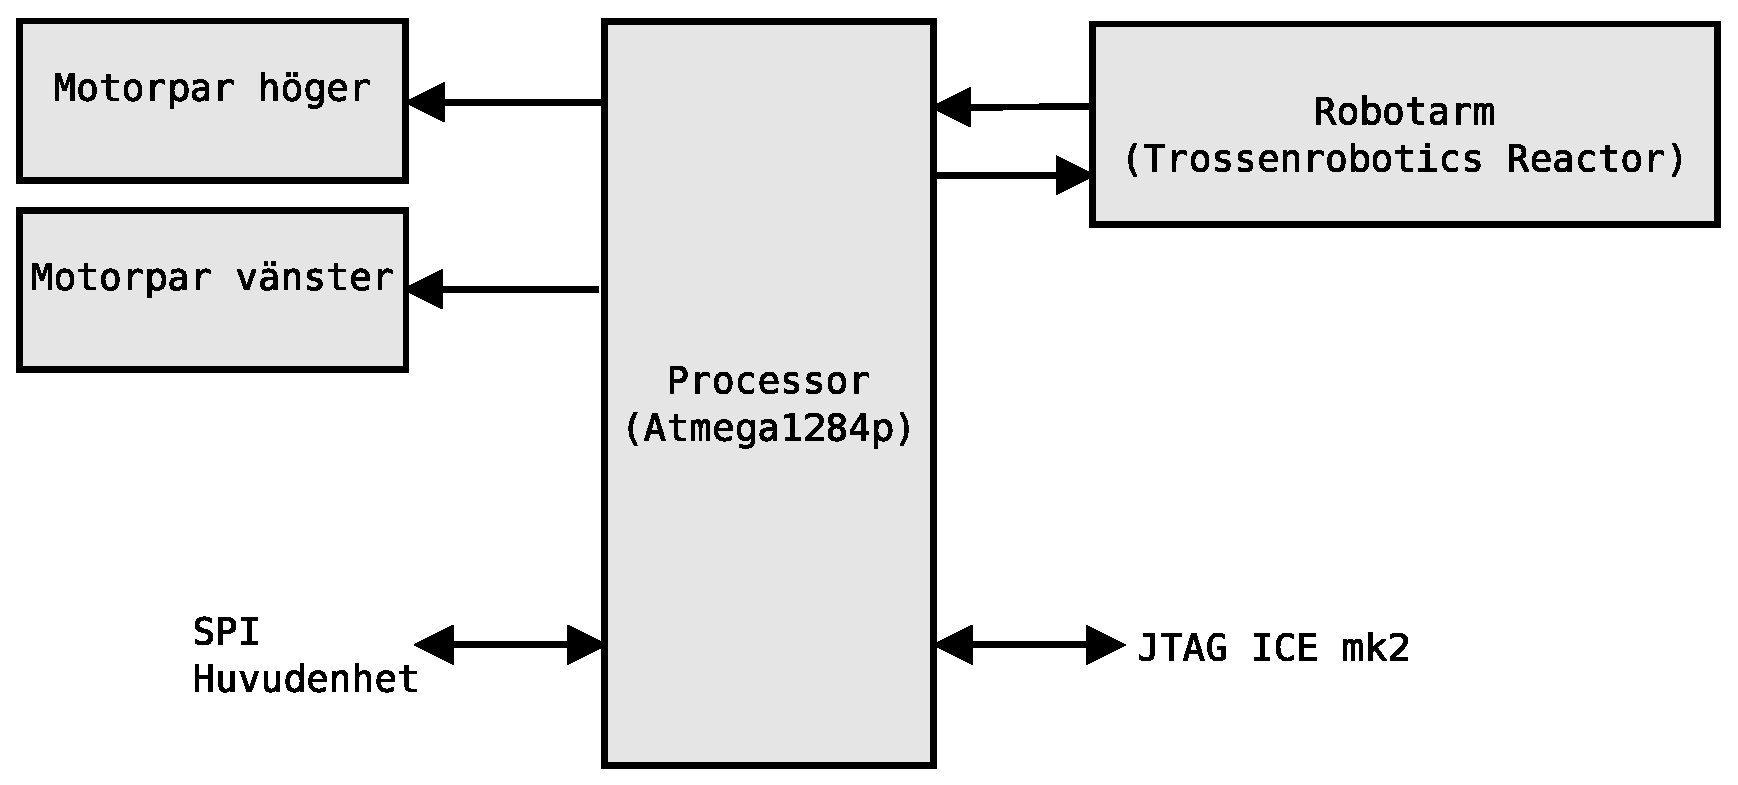
\includegraphics[scale=0.4]{grafik/styrenhet-oversikt}
	\caption{Översikt av styrenheten} \label{styr-oversikt}
\end{figure}

\subsubsection{Motorer}
Systemet har sammanlagt fyra motorer, uppdelat i två motorpar. De är anslutna till Styrenheten med en 10-pinnars flatkabel. Motorparen levererades med intelligenta H-bryggor\cite{pwmmotor} och behöver förses med en PWM-signal var, som bestämmer motorernas hastighet och en riktningssignal var där $1$ är i framriktningen och $0$ backriktningen.

\subsubsection{Robotarm}
Robotarmen är en Trossenrobotics Reactor och består av åtta servon av typ AX-12a\cite{servo}. Dessa är fördelade på fem axlar och en gripklo. De kommunicerar med Styrenheten över UART med en baudrate på 1MB/s, där både in och utsignal går via samma sladd. Denna är därför ansluten till två tristates för att förebygga att något oväntat skrivs eller läses från bussen.

\subsubsection{Processor}
Styrenheten drivs av en enkretsdator av typ Atmega1284p. Den kan anslutas till en PC via JTAG för att programmeras eller felsökas. Den har en klockfrekvens på 16MHz och tar emot kommandon från Huvudenheten, tolkar dessa och ser till att motorerna och robotarmen utför det som Huvudenheten har sagt. Figur \ref{styr-processor} visar hur enkretsdatorn är ansluten till övrig hårdvara.

\begin{figure}[h!]
	\centering
	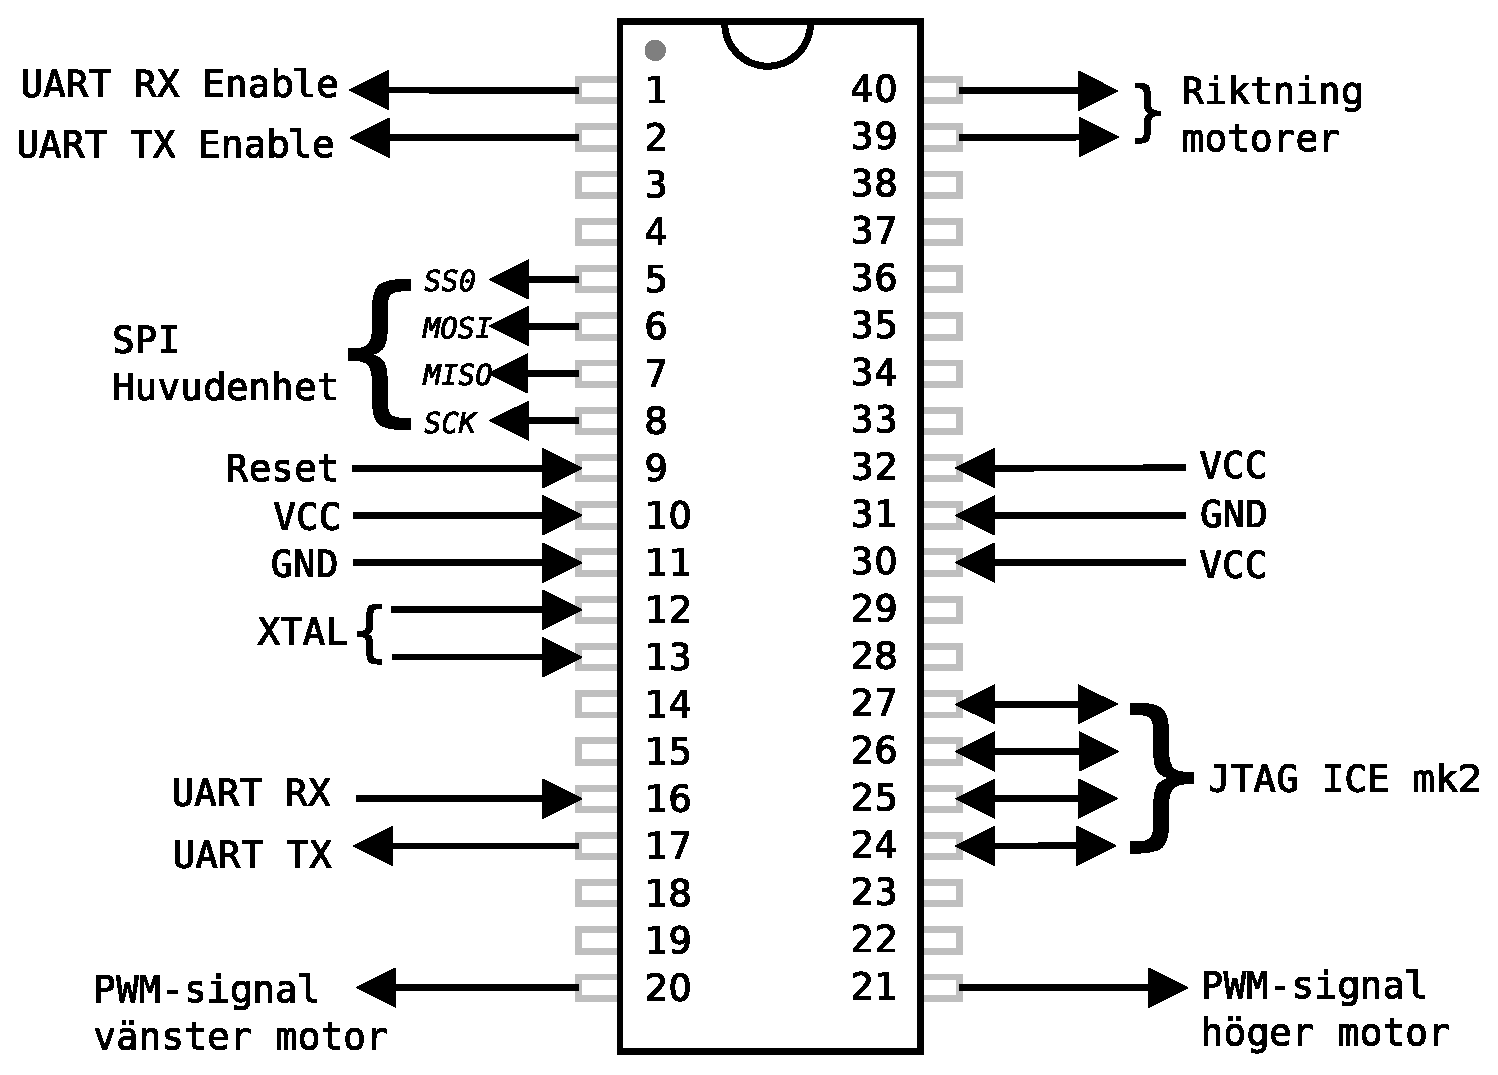
\includegraphics[scale=0.5]{grafik/styrenhet-processor}
	\caption{Schema över hur enkretssdatorn i styrenheten är ansluten till övrig hårdvara.} \label{styr-processor}
\end{figure}

\subsection{Mjukvara}
Styrenhetens mjukvara består av två moment. För det första tas kommandon emot via SPI från huvudenheten. Vi utnyttjar att Atmega1284p har hårdvarustöd för SPI och triggar ett interrupt när en byte tas emot.

\begin{figure}[h!]
	\centering
	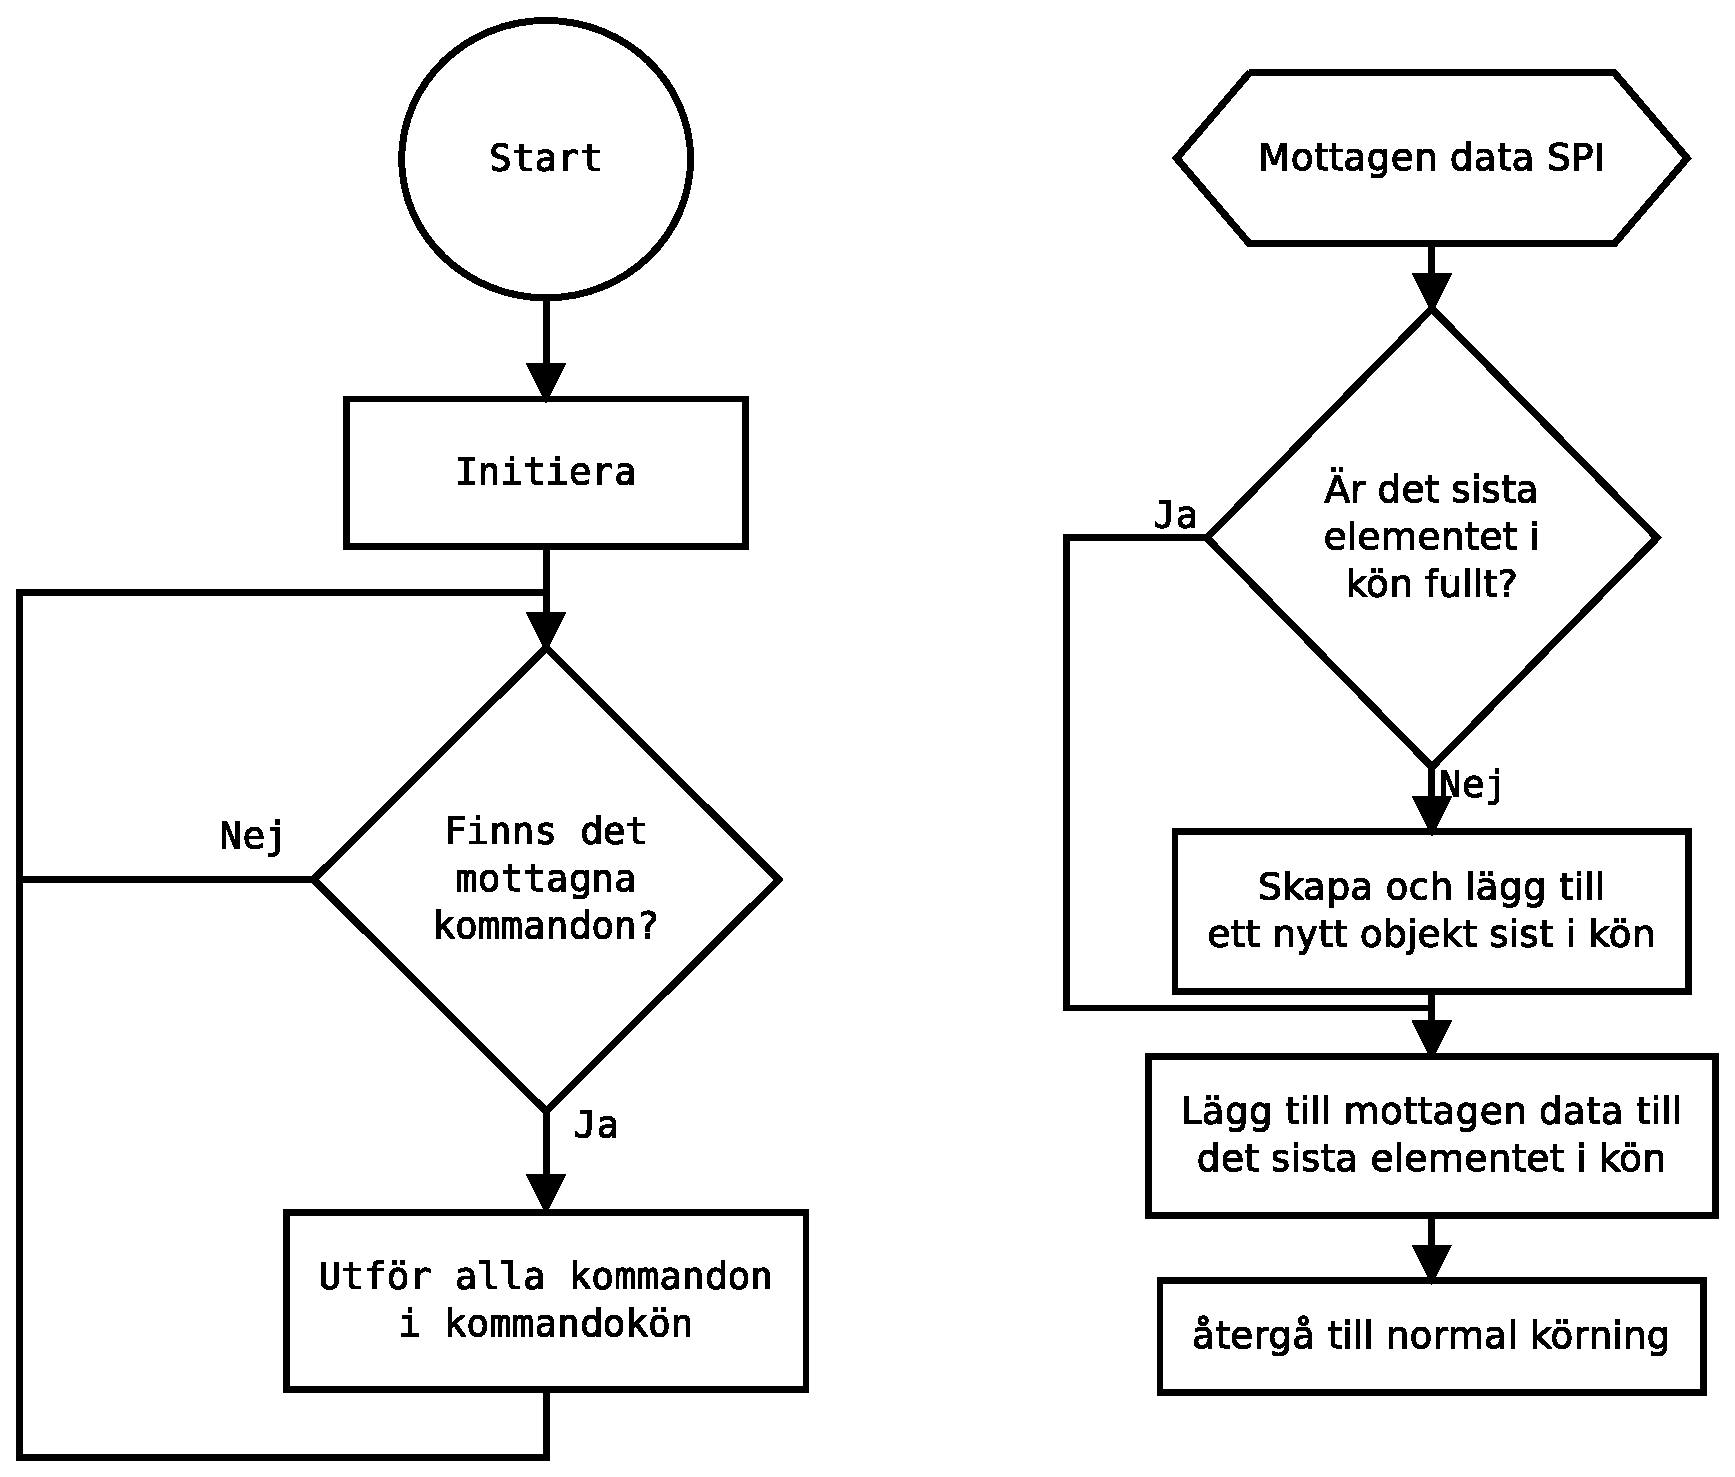
\includegraphics[scale=0.4]{grafik/styr-mjukvara}
	\caption{T.v. Styrenhetens mainloop. T.h. Hur styrenheten hanterar avbrott över SPI.} \label{styr-mjukvara}
\end{figure}

Centralt i mjukvaran är den kommandokö där mottagna databytes hamnar. Vi lägger alltid till inkomna databytes till det sista kommando-objektet i kön. Om vi får in en databyte och det sista objektet är fullt eller listan tom, skapas ett nytt kommando-objekt och läggs till kön. Vi vet att ett kommando-objekt är fullt genom att jämföra den förväntade längden (se \ref{protokoll-huvud-styr}) med hur många byte kommandot består av.

På andra sidan kommandokön har vi den del av mjukvaran som tolkar och utför inkomna kommandon. Den kollar kontinuerligt om kommandokön är tom. Är den inte det kollar vi om det första kommandoobjektet är fullt. Är det fullt mottaget tolkar vi och utför det.

Styrenheten kommunicerar med robotarmen över UART. Atmega1284p har hårdvarustöd för USART, vilket används genom att vi lägger till data till en buffert och väntar på att det skickas.

Motorernashastighet kontrolleras genom en PWM-signal till vardera motorpar. Vi utnyttjar att Atmega1284p har hårdvarustöd för två PWM-signaler som styrs av en timer var.

Styrenheten har en intern datatyp för typ av enhet den förväntas styra. Om det mottagna kommandot är ett av typen \texttt{Sätt register A till D} lagras detta i den adresserade hårdvarans datatyp. I det fall att det är armen som adresseras skickas den mottagna datan till rätt register med ett \texttt{WRITE}-kommando \cite{servo}. Det innebär att armen inte realiserar de mottagna värden förrän den får ett \texttt{ACTION}-kommando. När styrenheten mottager ett \texttt{Action}-kommando från huvudenheten realiserar den tidigare mottagna kommandon för den adresserade hårdvaran. Detta görs genom att skicka \texttt{ACTION}-kommandon till armen respektive sätter de timers som styr PWM-signalerna till motorparen.

% Hur är sensorenheten designad?

\section{Sensorenhet}

Sensorenheten har till uppgift att förse huvudenheten med sensordata. Sensordatan den returnerar är obehandlad rådata.

\subsection{Hårdvara}

%\begin{figure}[h!]
%	\centering
%	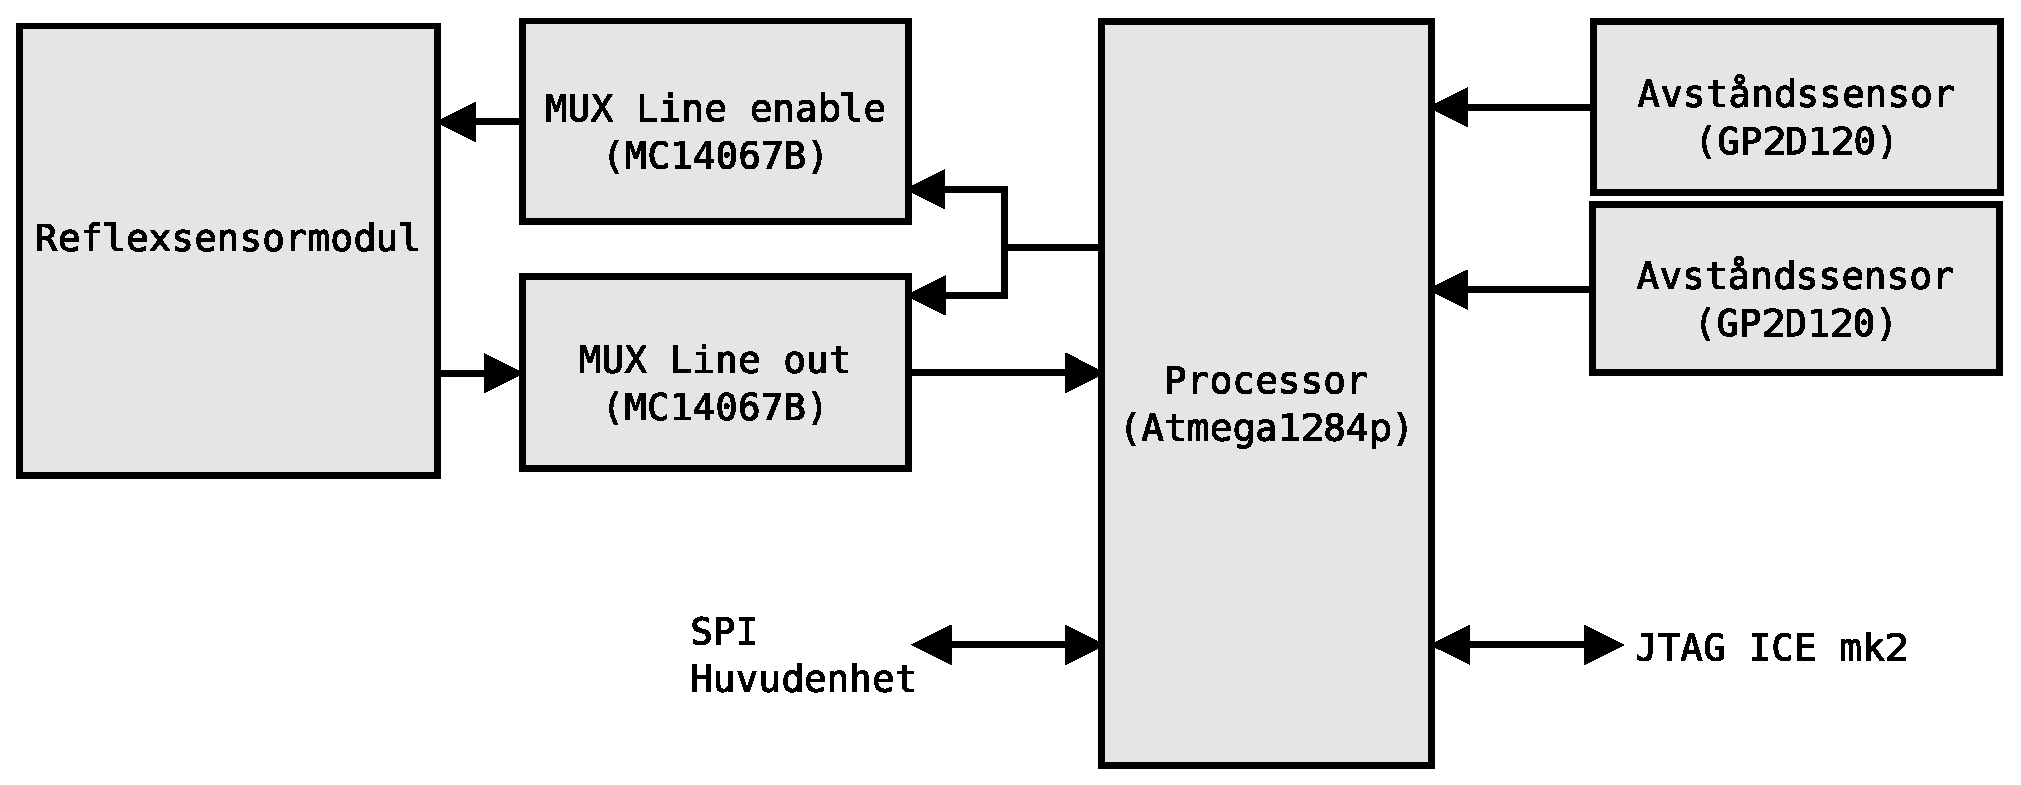
\includegraphics[scale=0.4]{grafik/sensorenhet-oversikt}
%	\caption{Översikt av sensorenheten }
%\end{figure}

Sensorenheten består av en Atmega1284p, en reflexsensormodul och två avståndssensorer. Reflexsensormodulen är kopplad via två 16-1 muxar till enkretsdatorn. Den ena muxen används för att styra en konstant hög enable-signal till rätt reflexsensor och den andra för att välja rätt utsignal. Båda muxarna styrs av samma styrsignal från processorn. Enkretsdatorn är ansluten till huvudenheten med en \todo{20lol-pinnarskabel?} över vilken de kommunicerar via SPI.

%\begin{figure}[h!]
%	\centering
%	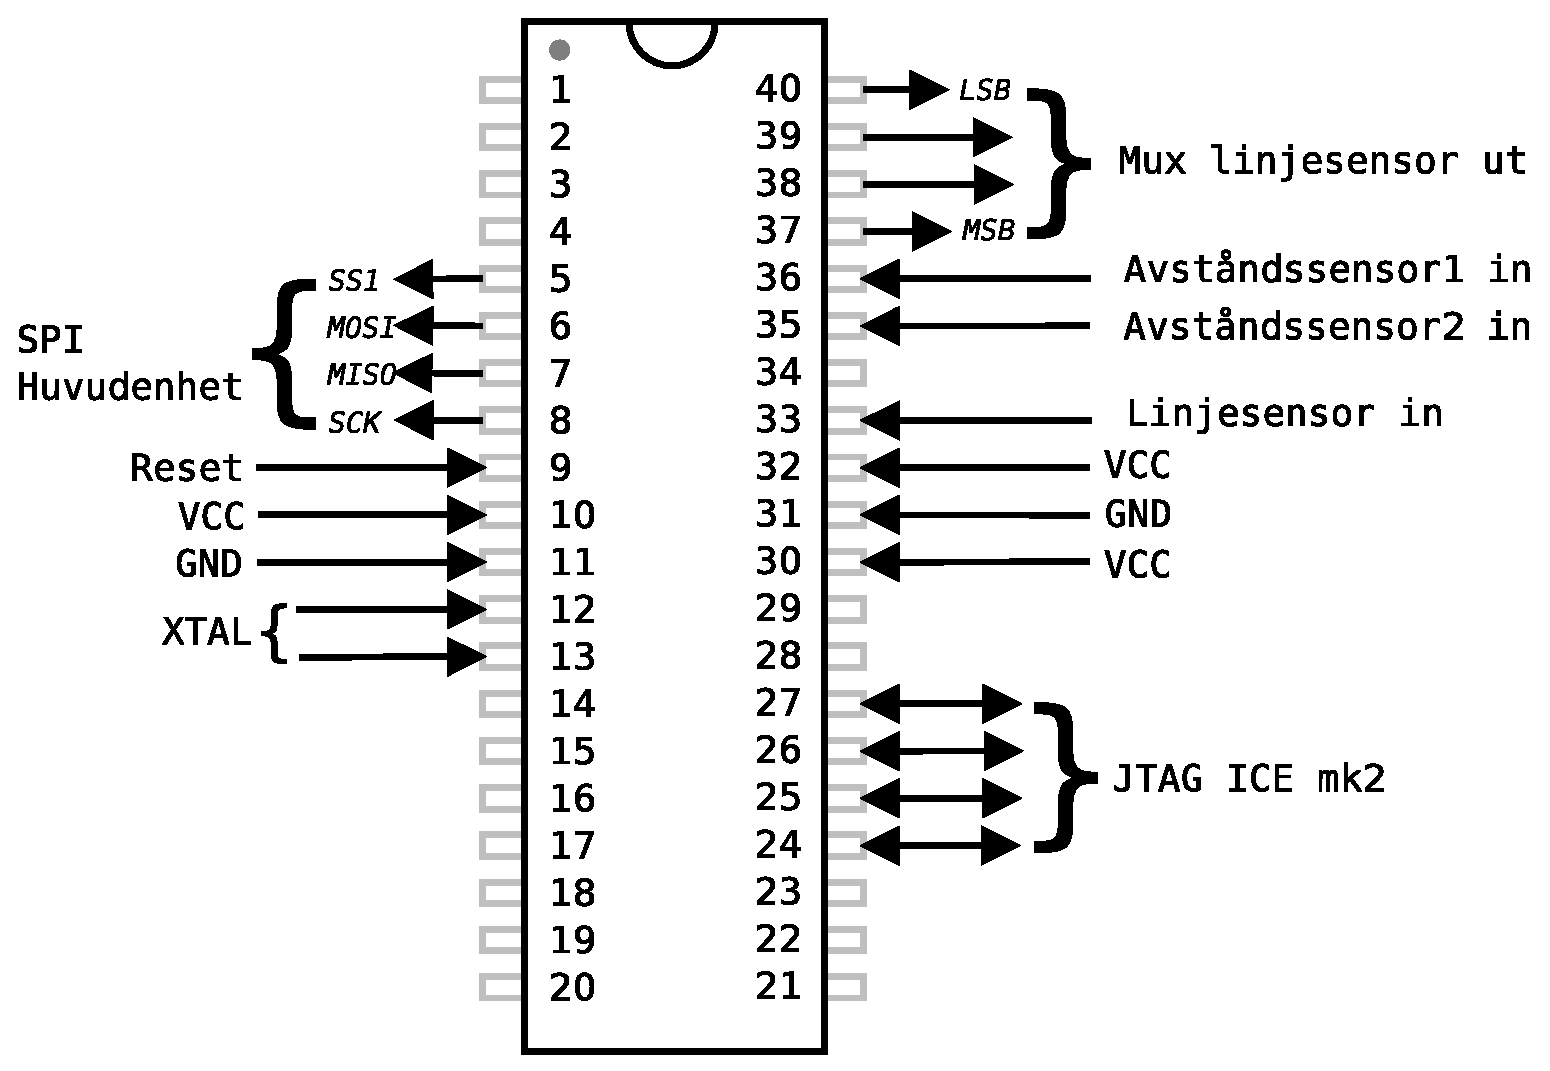
\includegraphics[scale=0.5]{grafik/sensorenhet-processor}
%	\caption{Schema över hur enkretssdatorn i sensorenheten är ansluten till övrig hårdvara.}
%\end{figure}

\subsubsection{Reflexsensormodul}

Reflexsensormodulens syfte är att detektera banan längs vilken roboten skall röra sig. Den består av 11 reflexsensorer som i sig består av en IR-diod och en fototransistor. Utsignalen ligger mellan 0V och 5V. De ger låg utspänning då underlaget reflekterar mycket ljus, och hög utspänning då lite ljus reflekteras.

\subsubsection{Avståndssensorer}

Avståndssensorerna är av typen GP2D120 vilken använder ljus för att detektera avståndet. Dess utsignal är en analog spänning mellan 0V och 3.2V.

\subsection{Mjukvara}

All mjukvara på sensorenheten är skriven i $C$ och finns på enkretsdatorn. Den består av två delar, illustrerat i figur \ref{sensorenhet-mjukvara}.

%\begin{figure}[h!]
%	\centering
%	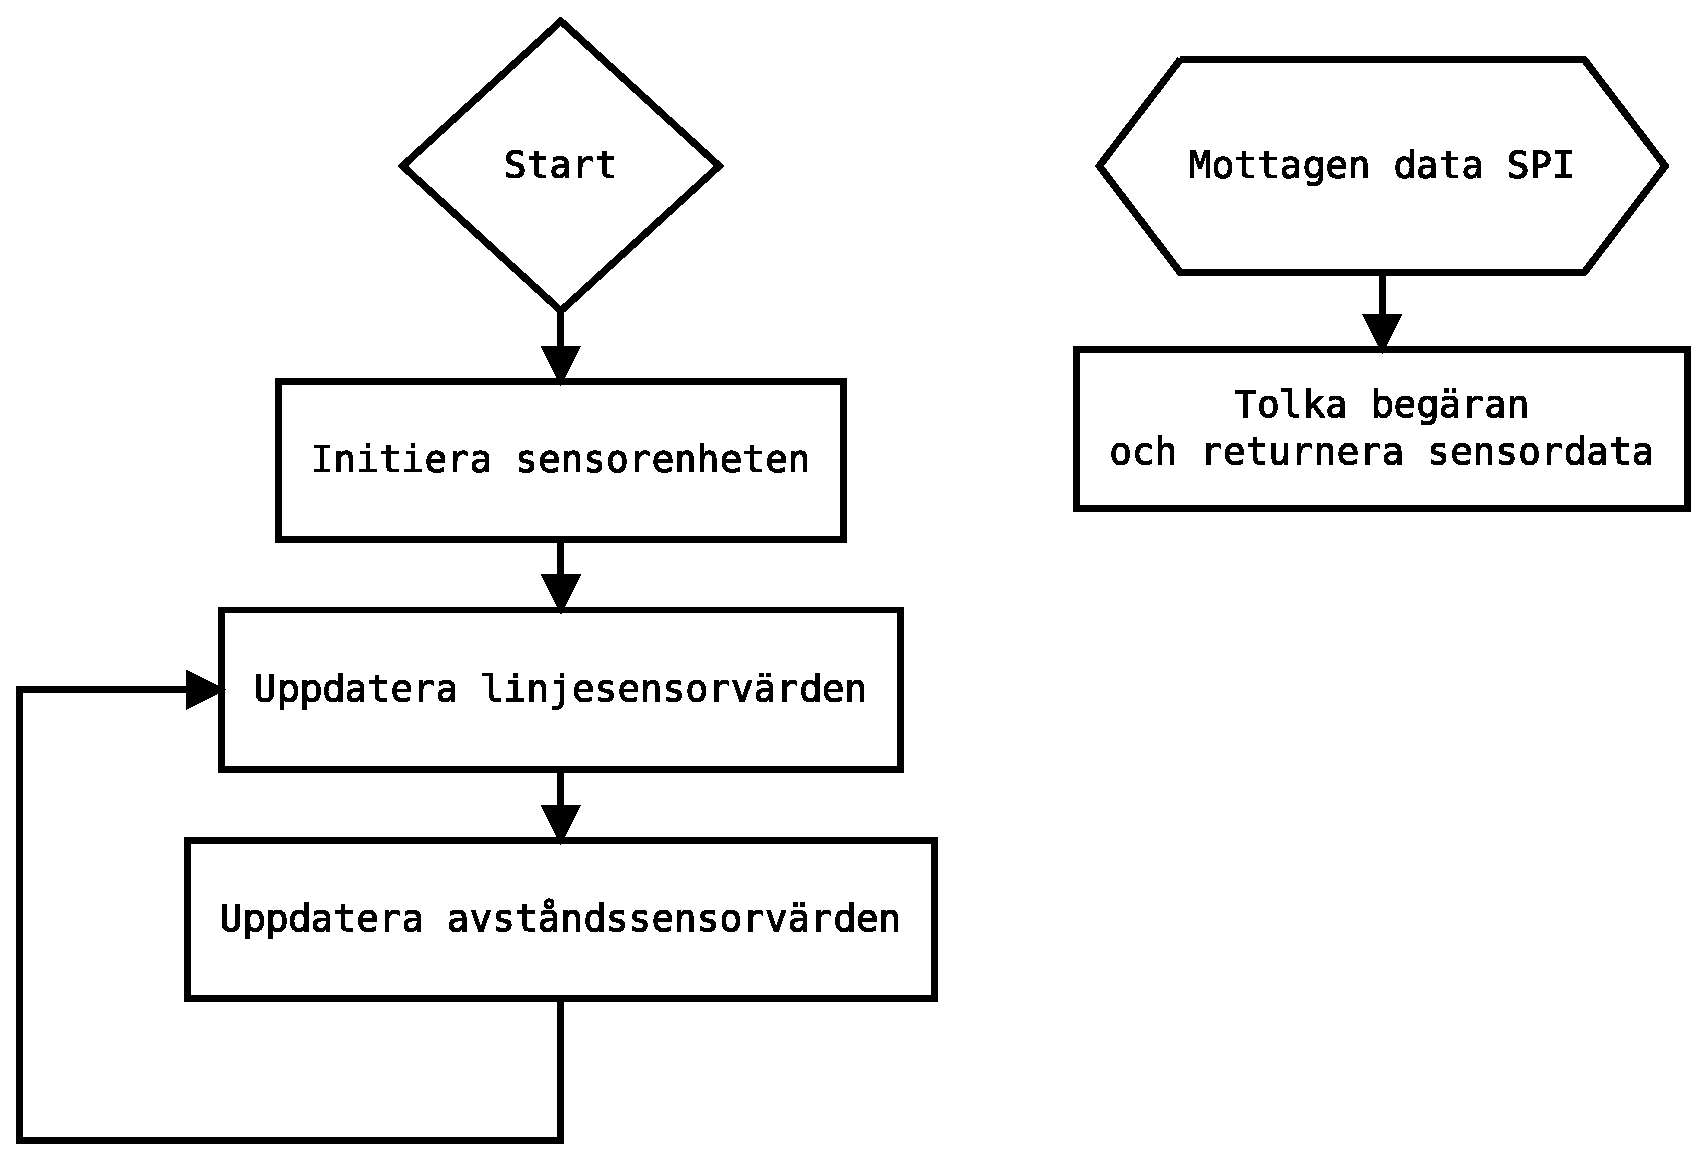
\includegraphics[scale=0.4]{grafik/sensorenhet-mjukvara}
%	\caption{Till vänster sensorenhetens \todo{huvudslinga}, till höger %den avbrottsrutin som körs vid mottagen data över SPI.} \label%{sensorenhet-mjukvara}
%\end{figure}

För det första körs en mainloop där sensordata kontinuerligt uppdateras. Först itererar vi igenom Reflexsensorerna genom att först styra om enable-signalen till den aktuella sensorn och därefter utföra en AD-omvandling på den signal vi får tillbaks och sedan gå till nästa. Därefter utför vi i tur och ordning en AD-omvandling på insignalerna från avståndssensorerna. Alla värden sparas i en global datastruktur.
\newline
För det andra tar sensorenheten emot begäran om sensordata från huvudenheten över SPI. När en sådan förfrågan inkommer triggas ett avbrott i vilket sensorenheten svarar med det aktuella sensorvärdet. Då inget i avläsningen av sensorerna är tidskritiskt behöver vi inte oroa oss för när dessa avbrott kommer.

% Analys av systemet. Vad kunde ha gjorts bättre? Vad kan utvecklas vidare?

\section{Slutsatser}

Vi har byggt en robot som kan utföra en rad uppgifter både autonomt och manuellt. Även om systemet fungerar felfritt så skulle många förbättrningar kunna göras.

Mjukvarumässigt kan en hel del kod optimeras för att systemet ska flyta på bättre, speciellt de delar där styrning av armen sker. På

beagleboarden återfinnes också kod för detta som kan göras bättre. Filtreringsfunktioner för sensorvärdena kan förbättras för att undvika felaktiga värden. All kod kan struktureras bättre för ökad läsbarhet.

Ur ett hårdvarumässigt perspektiv skulle fler och mer precisa sensorer (mer specifikt avståndssensorerna) kunna förbättra systemet.

Om vi hade haft mer tid hade vi önskat utöka funktionaliteten hos roboten. En autonom upplockning av paket hade varit önskvärd och hade gjort robotens autonoma läge helt komplett.

Som sagt fungerar systemet felfritt men med ovan nämnda förbättringar i mjukvaran samt hårdvaran kan produkten bli ännu mer attraktiv på marknaden.

\newpage
% Referenser

\begin{thebibliography}{9}
	\bibitem{servo}
	\url{http://support.robotis.com/en/techsupport_eng.htm#product/dynamixel/ax_series/dxl_ax_actuator.htm}, information hämtad 	2014-10-24
	\bibitem{atmega}
	\url{http://www.atmel.com/images/doc8059.pdf}, information hämtad \todo{hittepådatum}
	\bibitem{avstandsensor}
	\url{http://www.sharpsma.com/webfm_send/1205}, information hämtad \todo{Hittepådatum}
	\bibitem{ubuntu}
	\url{http://www.ubuntu.com}, Hur refererar vi ubuntu?}
	\bibitem{reflexsensormodul}
	\url{https://docs.isy.liu.se/twiki/pub/VanHeden/DataSheets/reflexsensormodul.pdf}, information hämtad \todo{hittepådatum}
	\bibitem{Muxar}
	\url{https://docs.isy.liu.se/twiki/pub/VanHeden/DataSheets/4067b.pdf}, information hämtad \todo{hittepådatum}
	\bibitem{tristate}
	\url{https://docs.isy.liu.se/twiki/pub/VanHeden/DataSheets/sn74ls125.pdf}, information hämtad \todo{hittepådatum}
	\bibitem{levelshifters}
	\url{http://www.ti.com/lit/ds/symlink/txb0104.pdf}, information hämtad \todo{hittepådatum}
\end{thebibliography}


%\todo{Datablad för atmega1284p} \newline
\todo{Resurs/datablad för Beagleboard?} \newline
%\todo{Datablad för GP2D120} \newline
%\todo{Datablad för reflexsensormodul + reflexsensorer} \newline
%\todo{Datablad för muxar} \newline
%\todo{Datablad för levelshifters} \newline
\todo{Datablad för kristall/oscillator} \newline
\todo{Datablad för tryckknapp} \newline
%\todo{Datablad för tri-state} \newline

%MUX - 4067 - https://docs.isy.liu.se/twiki/pub/VanHeden/DataSheets/4067b.pdf
%Tri-states - 74ls125
%Levelshifter - txb0104 - http://www.ti.com/lit/ds/symlink/txb0104.pdf
%tryckknapp - Cherry mx blå/röd/blun
%kristall - okänd


\newpage
\begin{appendices}

% Bilagor
\section{Kopplingsschema}

Nedan följer de kopplingsscheman som beskriver hur hårdvaran i Gloria hänger ihop.

\todo{Importera eagle-shit}


\end{appendices}


\end{document}
